\newpage
\chapter{METODE PENELITIAN} \label{chap:metode_penelitian}
\section{Alur Penelitian} \label{sec:alur_penelitian}
Tahapan penelitian ini dimulai dengan proses identifikasi masalah dan studi literatur untuk membangun landasan teori yang kuat. Selanjutnya, dilakukan pengumpulan data, anotasi data dan \textit{pre-processing}. Setelah data siap, penelitian berfokus pada pengembangan model arsitektur multimodal, yang kemudian diuji melalui tahap evaluasi model. Rangkaian penelitian ini diakhiri dengan analisis hasil dan pembahasan untuk menarik kesimpulan. Adapun ilustrasi lebih rinci mengenai alur penelitian ini dapat dilihat pada Gambar \ref{fig:alur_penelitian}. \par

\begin{figure}[H] % Kalau menggunakan H, posisi gambar akan tepat dibawah teks
    \centering
    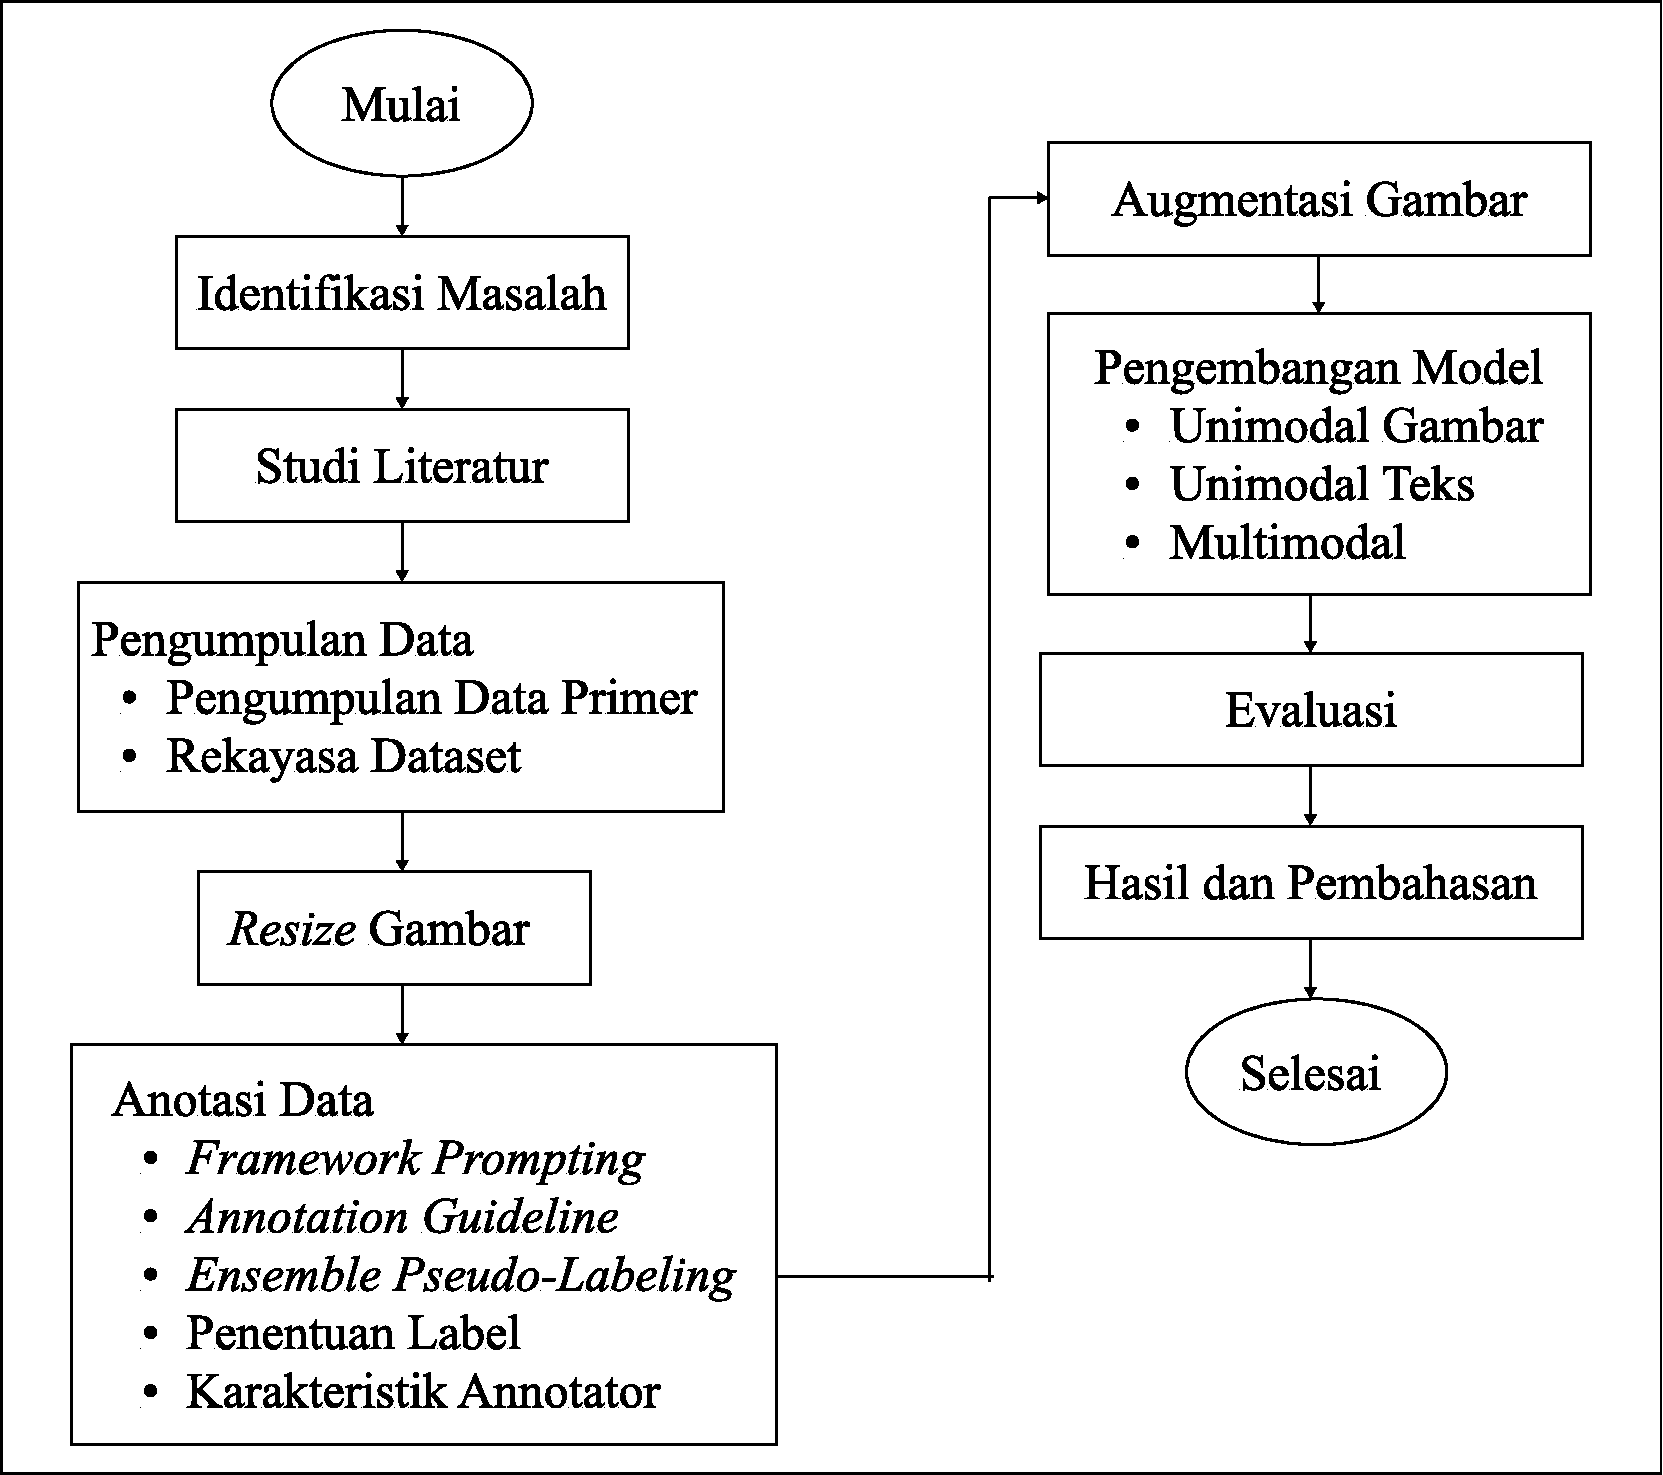
\includegraphics[width=0.9\textwidth]{figure/diagramalirrr.pdf}
    \caption{Alur Penelitian}
    \label{fig:alur_penelitian}
\end{figure}

\section{Penjabaran Langkah Penelitian} \label{sec:penjabaran_langkah_penelitian}
Pada alur penelitian yang telah digambarkan dalam diagram alur penelitian pada \ref{sec:alur_penelitian}, bagian ini menjelaskan secara rinci setiap tahapan yang dilakukan dalam penelitian. Penjabaran ini mencakup proses mulai dari pengumpulan data, anotasi, hingga tahap \textit{pre-processing} sebagai persiapan data. Selanjutnya, dijelaskan tahapan pengembangan model yang meliputi pembagian \textit{dataset}, pelatihan model, serta perancangan arsitektur multimodal. Tahap akhir yang diuraikan adalah evaluasi model untuk mengukur kinerja sistem dalam mengidentifikasi meme \textit{self-harm}.

\subsection{Identifikasi Masalah} \label{subsec:identifikasi_masalah}
Tahap pertama dalam penelitian ini adalah identifikasi masalah  melalui studi literatur, yang berfokus pada urgensi memahami meme dengan tema \textit{self-harm} sebagai bentuk konten digital yang memiliki makna implisit. Meme jenis ini sering menyampaikan pesan melalui kombinasi visual dan tekstual, seperti ironi, sarkasme, humor gelap, atau metafora, sehingga indikasi \textit{self-harm} tidak selalu tampak secara eksplisit dan memerlukan analisis multimodal untuk dapat dipahami secara utuh. Berdasarkan studi literatur, penelitian terkait deteksi meme berbahaya masih didominasi oleh kategori seperti ujaran kebencian, propaganda, dan konten ofensif, sementara meme dengan nuansa \textit{self-harm} masih sangat terbatas untuk diteliti. Hal ini disebabkan oleh keterbatasan ketersediaan \textit{dataset} publik yang relevan, sebagaimana diungkapkan oleh Sharma \textit{et al.}, yang menyatakan bahwa kurangnya \textit{dataset} menjadi hambatan utama dalam pengembangan penelitian pada domain meme berbahaya, khususnya untuk kategori yang kurang tereksplorasi seperti \textit{self-harm} \cite{Sharma2022HarmfulMemes}. Kondisi tersebut menunjukkan adanya kesenjangan riset yang mendorong perlunya pengembangan model multimodal yang mampu memahami hubungan antara teks dan gambar secara kontekstual dalam penelitian ini.

\subsection{Studi Literatur} \label{subsec:studi_literatur}
Tahap kedua dalam penelitian ini adalah studi literatur, yang mencakup kajian mendalam terhadap berbagai sumber ilmiah yang relevan dengan topik penelitian. Studi literatur ini bertujuan untuk memahami perkembangan metode dalam analisis konten multimodal, khususnya dalam mendeteksi meme berbahaya yang memiliki makna implisit melalui kombinasi teks dan gambar. Pada tahap ini, ditinjau penelitian terkait pemanfaatan \textit{large language models} sebagai \textit{automatic annotator} untuk mengatasi keterbatasan anotasi manual, kemampuan model multimodal dalam memahami emosi serta konteks visual dan tekstual, serta berbagai pendekatan deteksi \textit{harmful memes} yang umumnya memanfaatkan representasi visual dari model \textit{Contrastive Language-Image Pre-training} (CLIP). Selain itu, kajian literatur juga menyoroti keterbatasan penelitian pada domain meme \textit{self-harm} yang masih minim eksplorasi akibat keterbatasan \textit{dataset}, sehingga diperlukan pendekatan alternatif seperti \textit{pseudo-labeling} untuk membangun \textit{dataset} secara efisien. Hasil studi literatur tersebut menjadi landasan teoritis dalam merumuskan kesenjangan riset serta menyusun rancangan model multimodal yang diusulkan dalam penelitian ini.

\subsection{Pengumpulan Data} \label{subsec:pengumpulan_data}
Pengumpulan data merupakan tahap penting dalam penelitian ini untuk memperoleh data yang relevan dan mendukung proses analisis. Pada tahap ini, data yang dikumpulkan berupa meme multimodal yang terdiri dari kombinasi elemen visual dan tekstual. Proses pengumpulan data dilakukan dari berbagai sumber secara sistematis agar data yang diperoleh memiliki kualitas yang baik dan dapat dipertanggungjawabkan. Berikut merupakan metode pengumpulan data yang digunakan dalam penelitian ini.

\subsubsection{Pengumpulan Data Primer} \label{subsubsec:pengumpulan_data_primer}
Pada penelitian ini, data meme dikumpulkan secara manual dari beberapa platform media sosial, yakni Reddit, Instagram, Facebook, dan X. Pengumpulan manual dipilih karena meme merupakan unit multimodal (teks dan gambar) yang maknanya sering muncul dari interaksi kedua modalitas, sehingga pengambilan data harus mempertahankan format asli (gambar + teks dalam satu konteks). Hal ini sejalan dengan temuan survei \textit{harmful memes} yang menekankan bahwa konten berbahaya sering mengombinasikan beberapa modalitas dan tidak dapat dianalisis secara unimodal saja \cite{Sharma2022HarmfulMemes}. Proses pengumpulan dilakukan dengan memasukkan kata kunci atau tagar terkait \textit{self-harm} dan ideasi bunuh diri pada fitur pencarian masing-masing platform. Daftar hashtag yang digunakan dalam proses pengumpulan data dapat dilihat pada Tabel~\ref{tabel:hashtag_pengumpulan_data}.

\begin{table}[H]
    \centering
    \caption{Daftar Hashtag Pengumpulan Data Primer}
    \label{tabel:hashtag_pengumpulan_data}
    \small
    \setlength{\tabcolsep}{8pt}
    \renewcommand{\arraystretch}{1.1}
    \begin{tabular}{c l}
        \hline
        \textbf{No} & \textbf{Hashtag} \\
        \hline
        1 & \#selfharm \\
        2 & \#selfharmmm \\
        3 & \#killmyself \\
        4 & \#iwannacutmyself \\
        5 & \#suicidal \\
        6 & \#depression \\
        7 & \#sad \\
        8 & \#broken \\
        9 & \#tiredoflife \\
        10 & \#numb \\
        11 & \#overthinking \\
        12 & \#pain \\
        13 & \#mentalhealth \\
        14 & \#hopeless \\
        15 & \#worthless \\
        \hline
    \end{tabular}
\end{table}


Strategi pencarian berbasis kata kunci dipandang relevan karena literatur menunjukkan adanya proliferasi konten \textit{self-harm} di media sosial dan efek normalisasi yang bisa meningkat karena paparan berulang \cite{MoraledaEsteban2025SelfHarm}. Pengumpulan manual ini memungkinkan peneliti untuk menyeleksi meme yang secara eksplisit atau implisit mengandung indikasi \textit{self-harm}, sehingga dataset yang diperoleh lebih sesuai dengan tujuan penelitian. Dalam proses seleksi, konten dipilih berdasarkan kriteria sebagai berikut:
\begin{enumerate}
    \item Memuat kombinasi teks dan gambar, atau teks yang ditempel pada gambar sehingga dapat dianalisis secara multimodal.
    \item Konteks meme masih dapat dipahami dengan jelas.
    \item Mengandung indikasi \textit{self-harm}, baik secara eksplisit maupun implisit.
\end{enumerate}
Proses pengumpulan data ini menghasilkan sebanyak 268 meme \textit{self-harm}. Data tersebut kemudian diproses lebih lanjut pada tahap anotasi sebelum digunakan dalam pelatihan model multimodal.

\subsubsection{Rekayasa Dataset Meme \textit{Self-Harm}} \label{subsubsec:rekayasa_dataset_meme_self_harm}
Selain pengumpulan data melalui media sosial, penelitian ini melakukan rekayasa dataset untuk memperkaya variasi contoh \textit{self-harm} dan meningkatkan keberagaman pola multimodal yang dapat dipelajari model. Langkah ini juga didorong oleh literatur \textit{harmful memes} yang menyatakan bahwa beberapa kategori \textit{harmful memes}, termasuk meme yang memuat \textit{self-harm}, masih kurang diteliti karena keterbatasan dataset yang sesuai \cite{Sharma2022HarmfulMemes}. 

Rekayasa dataset dilakukan dengan membangun meme multimodal secara manual melalui penggabungan komponen tekstual dari dataset publik \textit{Suicidal Ideation Detection Reddit Dataset} yang berisi postingan Reddit dengan label \textit{suicidal} dan \textit{non-suicidal}, serta komponen visual dari dataset publik bertipe \textit{object detection} yang memuat objek berbahaya pisau dan senjata api \cite{mafi_alam_2023_suicidal_reddit}\cite{ali_weapon_knife_2025}. Gambar-gambar tersebut dipilih untuk merepresentasikan \textit{visual cues} yang secara umum diasosiasikan dengan risiko kekerasan atau cedera tanpa harus menampilkan luka eksplisit.

Komponen teks dalam penelitian ini dipilih dari subset teks berlabel \textit{suicidal} dengan tingkat kejelasan (\textit{confidence}) yang tinggi terhadap indikasi keputusasaan, serta menghindari teks yang terlalu pendek atau ambigu. Penggunaan teks \textit{suicidal} tidak dimaksudkan untuk menyamakan konsep \textit{suicidal} dengan \textit{self-harm}, melainkan karena keduanya memiliki keterkaitan dalam spektrum ekspresi \textit{distress} psikologis dan sama-sama memancarkan sinyal negatif yang relevan untuk analisis risiko. Oleh karena itu, teks dengan indikasi \textit{suicidal} digunakan sebagai pendekatan untuk merepresentasikan sinyal linguistik yang mendekati konteks \textit{self-harm} dalam meme sintetis. Pemilihan ini bertujuan untuk membentuk meme sintetis yang secara semantik lebih konsisten dengan indikator risiko \textit{self-harm}. Pertimbangan tersebut diperkuat oleh tinjauan sistematis yang menunjukkan bahwa paparan konten \textit{self-harm}, bahkan tanpa representasi luka eksplisit, tetap dapat memicu berbagai dampak berbahaya seperti eskalasi \textit{self-harm}, \textit{social comparison}, dan terbentuknya \textit{self-harm identity} \cite{Susi2023ViewingSelfHarmImages}. Dengan demikian, kekuatan sinyal dalam konten, termasuk teks, menjadi faktor penting dalam membedakan konten berisiko tinggi dan rendah.

Rekayasa dataset ini menghasilkan 524 meme \textit{self-harm} sintetis. Seluruh meme sintetis tersebut diperlakukan sebagai data penelitian yang harus melalui proses anotasi dan tidak otomatis dianggap benar, sehingga label akhir tetap ditentukan berdasarkan \textit{annotation guideline} yang disusun berbasis literatur melalui \textit{pseudo-labelling} oleh \textit{large language model} yang akan dijelaskan dalam sub bab anotasi data.

\subsubsection{Dataset Meme Umum sebagai Kandidat \textit{Non-Self-Harm}} \label{subsubsec:dataset_meme_umum_non_self_harm}
Selain data \textit{self-harm} yang dikumpulkan secara langsung dari media sosial dan data hasil rekayasa dataset, penelitian ini juga menggunakan sebanyak 1.500 meme yang diambil dari dataset publik \textit{``6992 Labeled Meme Images Dataset''}. Dataset ini dikembangkan untuk keperluan analisis sentimen dan klasifikasi meme multimodal, sehingga memuat berbagai konteks humor umum, ekspresi emosi sehari-hari, serta interaksi sosial yang lazim ditemukan di internet \cite{javaid_6992_meme_images_2023}.

Dataset tersebut tidak secara eksplisit dirancang untuk tugas klasifikasi \textit{self-harm}. Oleh karena itu, secara konseptual dataset ini dapat mengandung konten yang bersifat netral maupun konten yang berpotensi ambigu. Dalam penelitian ini, dataset tersebut tidak diasumsikan sebagai \textit{non-self-harm}, melainkan diperlakukan sebagai kumpulan data kandidat yang diharapkan mayoritas merepresentasikan konten \textit{non-self-harm}. Pemilihan dataset meme umum ini bertujuan untuk menyediakan \textit{baseline} konten netral serta memperkaya distribusi data selama proses \textit{pseudo-labeling}. Label akhir dari setiap meme dalam dataset ini ditentukan pada tahap anotasi data menggunakan \textit{annotation guideline} berbasis literatur dan pendekatan \textit{ensemble pseudo-labeling}. Dengan demikian, jumlah data yang pada akhirnya dilabeli sebagai \textit{non-self-harm} maupun \textit{self-harm} baru dapat dipastikan setelah seluruh proses anotasi selesai. Pendekatan ini sejalan dengan praktik \textit{weak supervision}, dimana data mentah yang belum memiliki label spesifik dimasukkan ke dalam \textit{pipeline} anotasi dan pelabelan otomatis, kemudian ditentukan kelas akhirnya melalui agregasi beberapa sumber pelabelan, bukan berdasarkan asumsi awal \cite{ratner2019}.


\subsection{\textit{Pre-processing} Awal} \label{subsec:preprocessing_awal}
\textit{Pre-processing} awal dilakukan sebelum tahap anotasi data dengan tujuan untuk menyiapkan data agar lebih efisien dalam proses pemrosesan multimodal. Tahap ini berfokus pada penyeragaman ukuran data serta pengurangan kompleksitas komputasi tanpa menghilangkan informasi penting yang terkandung dalam meme. Pada tahap ini, seluruh gambar diubah ukurannya menjadi 224$\times$224 piksel untuk mengurangi kebutuhan komputasi dan biaya pemrosesan, dengan tetap menjaga keterbacaan teks yang terdapat pada meme.

Pemilihan ukuran 224$\times$224 piksel juga disesuaikan dengan kebutuhan \textit{input} model \textit{vision encoder} CLIP yang digunakan dalam penelitian ini, sehingga data yang dihasilkan kompatibel dengan arsitektur model tanpa memerlukan penyesuaian tambahan pada tahap pelatihan. Selain itu, ukuran ini mempertimbangkan keseimbangan antara efisiensi pemrosesan dan kualitas informasi visual, sehingga baik elemen gambar maupun teks tetap dapat dianalisis dengan baik oleh model \textit{vision-language}. Dengan demikian, proses \textit{pre-processing} awal ini memastikan bahwa data yang digunakan pada tahap anotasi memiliki format yang seragam, lebih ringan untuk diproses, serta tetap merepresentasikan konten multimodal secara optimal.

\subsection{Anotasi Data} \label{subsec:anotasi_data}
Tahap anotasi data dalam penelitian ini menggunakan pendekatan \textit{ensemble pseudo-labeling} dengan memanfaatkan dua model \textit{vision-language}, yaitu GPT-4o mini dan Qwen-VL-Flash, untuk menghasilkan label biner \textit{self-harm} dan \textit{non self-harm} pada meme multimodal. Pendekatan ini memanfaatkan kemampuan analisis multimodal dari kedua model dalam memahami hubungan antara elemen visual dan tekstual, sehingga diharapkan dapat meningkatkan akurasi pelabelan.

Proses anotasi menghasilkan \textit{output}, yaitu \textit{filename}, teks terlihat, label, serta relasi antara gambar dan teks. Teks terlihat berfungsi sebagai representasi teks yang diekstraksi langsung dari gambar dan digunakan sebagai pengganti proses \textit{optical character recognition} (OCR) pada tahap pelatihan model. Sementara itu, komponen relasi gambar dan teks digunakan untuk mendukung proses peninjauan ulang secara manual, terutama pada kasus yang bersifat ambigu.

Kedua model, yaitu GPT-4o mini dan Qwen-VL-Flash, menghasilkan \textit{output} dengan format yang seragam untuk setiap data. Apabila kedua model menghasilkan label yang konsisten, maka label tersebut digunakan sebagai label akhir. Namun, apabila terjadi perbedaan (\textit{disagreement}), dilakukan proses peninjauan ulang secara manual oleh peneliti dengan mengacu pada \textit{annotation guideline}. Pada tahap ini, dilakukan pula verifikasi terhadap teks terlihat untuk memastikan kesesuaiannya dengan teks asli pada gambar. Berdasarkan hasil evaluasi selama proses anotasi, \textit{output} OCR dari GPT-4o mini menunjukkan tingkat kesesuaian yang lebih tinggi dibandingkan Qwen-VL-Flash. Oleh karena itu, pada \textit{dataset} final, komponen teks yang digunakan dalam pelatihan model diambil dari hasil ekstraksi GPT-4o mini. Penjelasan lebih lanjut mengenai \textit{prompting} dan \textit{annotation guideline} disajikan pada subbab berikutnya. Distribusi label akhir yang dihasilkan dari proses anotasi ini disajikan pada Bab IV.

\subsubsection{\textit{Framework Prompting} (\textit{RapGuard})} \label{subsubsec:framework_prompting_rapguard}
Kerangka \textit{RapGuard} digunakan untuk menangani kompleksitas analisis meme yang memadukan teks dan gambar, sebagai dasar dalam perancangan \textit{prompting} yang digunakan ke \textit{large language model}. Kerangka ini digunakan karena metode \textit{prompting} sederhana atau statis pada umumnya hanya menganalisis teks atau gambar secara terpisah, sehingga berpotensi mengabaikan risiko yang baru muncul ketika kedua modalitas tersebut digabungkan. \textit{RapGuard} secara khusus dirancang untuk mendorong model melakukan analisis terstruktur terhadap tiga aspek utama, yaitu konten visual, konten tekstual, serta hubungan antara teks dan gambar. Selain itu, kerangka ini juga menyertakan tahap \textit{self-checking}, dimana model diminta untuk meninjau kembali keputusan awalnya secara kritis sebelum memberikan label akhir. Pendekatan ini bertujuan untuk meningkatkan keandalan pelabelan, terutama pada kasus meme yang bersifat ambigu, menggunakan humor gelap, atau menyembunyikan makna berbahaya secara implisit \cite{Jiang2024RapGuard}. Dengan demikian, penggunaan \textit{RapGuard} memungkinkan proses anotasi dilakukan secara lebih sistematis dan konsisten, tanpa penilaian tunggal terhadap satu modalitas.


\subsubsection{\textit{Annotation Guideline} Berbasis Literatur} \label{subsubsec:annotation_guideline_berbasis_literatur}
\textit{Annotation guideline} dalam penelitian ini disusun berdasarkan studi literatur dan dirancang untuk memastikan proses anotasi dilakukan secara sistematis dan konsisten. \textit{Guideline} ini terdiri dari tiga tahap analisis utama, yaitu analisis visual, analisis tekstual, dan analisis relasional yang berfokus pada hubungan antara gambar dan teks dalam meme. Analisis ini dirancang mengikuti kerangka \textit{RapGuard} yang menekankan pentingnya memahami interaksi antara modalitas visual dan tekstual dalam meme, sehingga dapat mengidentifikasi indikasi \textit{self-harm} yang mungkin tersembunyi secara implisit.

Indikator \textit{self-harm} dalam penelitian ini dibagi menjadi dua kategori utama, yaitu indikator naratif/tekstual dan indikator visual/simbolik. Indikator tersebut mencakup berbagai aspek, seperti deskripsi metode, ideasi kematian, romantisasi \textit{self-harm}, keberadaan objek berbahaya, representasi luka fisik, serta kontras ironis antara visual dan teks yang memperkuat makna implisit \cite{Wijaya2024SelfDiagnose}. Aturan pelabelan dalam \textit{guideline} ini adalah suatu meme diklasifikasikan sebagai \textit{self-harm} apabila memenuhi minimal satu indikator yang relevan, khususnya indikator relasional yang menunjukkan keterkaitan antara teks dan gambar. Selain itu, proses anotasi juga dilengkapi dengan tahap \textit{self-checking} untuk mengurangi subjektivitas dalam interpretasi meme yang bersifat ambigu. Rincian lengkap mengenai \textit{annotation guideline} yang digunakan dalam penelitian ini disajikan pada Lampiran.


\subsubsection{\textit{Ensemble Pseudo-Labeling}} \label{subsubsec:ensemble_pseudo_labeling}
Proses pelabelan dilakukan menggunakan pendekatan \textit{ensemble pseudo-labeling} dengan dua model \textit{vision-language}, yaitu GPT-4o dan Qwen-VL-Flash. 
Seluruh data dianotasi secara independen oleh kedua model menggunakan \textit{prompt} dan \textit{annotation guideline} yang sama. Apabila kedua model menghasilkan label yang sama, label tersebut diterima sebagai label akhir. Namun, apabila terdapat perbedaan label antara kedua model, data tersebut ditinjau ulang secara manual oleh peneliti berdasarkan \textit{annotation guideline} untuk menentukan label akhir.

\subsubsection{Penentuan Label} \label{subsubsec:penentuan_label}
Perbedaan hasil pelabelan antara dua model dapat terjadi pada beberapa sampel meme. Dalam kondisi tersebut, dilakukan peninjauan ulang secara manual oleh peneliti untuk menetapkan label akhir. Proses ini bertujuan untuk memastikan bahwa keputusan pelabelan tidak hanya bergantung pada satu hasil prediksi model, melainkan mempertimbangkan analisis. Penetapan label akhir mengacu pada indikator yang telah ditetapkan dalam \textit{annotation guideline} berbasis studi literatur, serta mempertimbangkan keluaran tambahan berupa relasi antara gambar dan teks yang dihasilkan oleh masing-masing model. Selain itu, hasil ekstraksi teks terlihat juga diverifikasi untuk memastikan kesesuaiannya dengan teks asli pada gambar, sehingga analisis yang dilakukan benar-benar merepresentasikan konten aktual pada meme.

Meme diklasifikasikan sebagai \textit{self-harm} apabila memenuhi setidaknya satu indikator yang berkaitan dengan \textit{self-harm}, khususnya indikator relasional yang menunjukkan keterkaitan antara teks dan gambar. Sebaliknya, meme diklasifikasikan sebagai \textit{non self-harm} apabila tidak ditemukan indikator yang relevan dan konteks yang ditampilkan hanya berupa humor umum atau ekspresi sehari-hari. Pendekatan ini digunakan untuk meminimalkan kemungkinan konten berisiko tidak teridentifikasi, sekaligus tetap mempertimbangkan karakteristik meme yang sering menyampaikan makna secara implisit melalui humor, ironi, atau metafora.


\subsubsection{Karakteristik \textit{Annotator}} \label{subsubsec:karakteristik_annotator}
Dalam penelitian ini, tahap evaluasi dilakukan dengan membandingkan hasil prediksi model terhadap label yang diberikan oleh manusia (\textit{human annotation}) sebagai \textit{ground truth}. Oleh karena itu, kualitas dan karakteristik \textit{annotator} menjadi aspek penting yang perlu dijelaskan, karena dapat memengaruhi interpretasi terhadap konten meme yang bersifat multimodal dan ambigu.

\begin{table}[H]
    \centering
    \caption{Karakteristik \textit{Annotator}}
    \label{table:4.karakteristik_annotator}
    \small
    \setlength{\tabcolsep}{4pt}
    \renewcommand{\arraystretch}{1.2}
    \begin{tabular}{>{\centering\arraybackslash}m{2.8cm} >{\centering\arraybackslash}m{2.6cm} >{\centering\arraybackslash}m{2.7cm}}
        \hline
        \textbf{Aspek} & \textbf{Annotator 1} & \textbf{Annotator 2} \\
        \hline
        Pekerjaan & Dosen & Mahasiswa \\
        Usia & 33 & 20 \\
        Gender & Laki-laki & Perempuan \\
        \hline
    \end{tabular}
\end{table}

Kedua \textit{annotator} memiliki latar belakang yang berbeda, baik dari sisi pekerjaan maupun gender, sehingga diharapkan dapat merepresentasikan variasi interpretasi manusia terhadap konten meme. \textit{Annotator} pertama memiliki latar belakang di bidang teknologi informasi (IT) dan sudah terbiasa dengan meme, sedangkan \textit{annotator} kedua berasal dari latar belakang non-IT dan belum terbiasa dengan meme. Sebelum proses anotasi dilakukan, kedua \textit{annotator} diberikan \textit{annotation guideline} yang sama sebagai acuan dalam melakukan pelabelan. \textit{Guideline} ini mencakup analisis visual, tekstual, serta hubungan antara keduanya dalam memahami makna meme secara multimodal. Proses anotasi dilakukan secara independen (\textit{blind annotation}), masing-masing \textit{annotator} tidak memiliki akses terhadap hasil anotasi \textit{annotator} lainnya. Pendekatan ini bertujuan untuk meminimalkan bias serta memastikan bahwa setiap keputusan anotasi merepresentasikan interpretasi individu secara objektif \cite{Perdana2025MultitaskNLU}.

Dalam penelitian ini, interpretasi terhadap konten tidak bersifat absolut dan dapat dipengaruhi oleh perspektif individu. Meskipun tingkat familiaritas \textit{annotator} terhadap budaya meme tidak secara eksplisit diukur dalam penelitian ini, penggunaan \textit{annotation guideline} yang terstandarisasi bertujuan untuk menjaga konsistensi proses pelabelan. Dengan demikian, variasi latar belakang \textit{annotator} tetap dapat dimanfaatkan untuk menangkap keberagaman interpretasi manusia.


\subsection{Augmentasi Gambar} \label{subsubsec:augmentasi_gambar}
Augmentasi gambar merupakan teknik yang digunakan untuk meningkatkan variasi data pelatihan dengan memodifikasi data yang ada tanpa mengubah makna utamanya. Teknik ini penting untuk membantu model dalam mempelajari pola yang lebih general serta mengurangi risiko \textit{overfitting}. Dalam penelitian ini, augmentasi diterapkan pada modalitas gambar untuk meningkatkan kemampuan model dalam mengenali pola visual pada berbagai kondisi. Augmentasi dilakukan secara acak pada data latih. Penerapan augmentasi ini bertujuan agar model tidak bergantung pada pola visual tertentu, seperti orientasi atau kondisi pencahayaan tertentu serta untuk menambah variasi data latih. Dengan demikian, model diharapkan menjadi lebih \textit{robust} terhadap variasi visual yang umum ditemukan pada meme.

\subsubsection{\textit{Flip}} \label{subsubsubsec:flip}
\textit{Flipping horizontal} diterapkan pada gambar untuk meningkatkan kemampuan model dalam mengenali objek dari berbagai orientasi. Pada tahap ini, gambar dibalik secara acak secara horizontal dengan probabilitas 50\%. Teknik ini memungkinkan model untuk tidak bergantung pada orientasi tertentu, sehingga model tetap dapat mendeteksi objek meskipun posisinya berubah, seperti ketika objek menghadap ke kiri atau kanan. Contoh dari augmentasi ini dapat dilihat pada Gambar \ref{fig:perbandingan_flip}, yang menunjukkan perbandingan antara gambar asli dan hasil augmentasi.
\begin{figure}[H]
    \centering
    % Gambar 1: Asli
    \begin{subfigure}[b]{0.45\textwidth}
        \centering
        
\includegraphics[width=0.7\textwidth]{figure/gambarasli.jpg}
        \caption{Gambar asli}
        \label{fig:gambar_asli_flip}
    \end{subfigure}
    \hspace{0.05\textwidth}
    % Gambar 2: Flip Horizontal
    \begin{subfigure}[b]{0.45\textwidth}
        \centering
        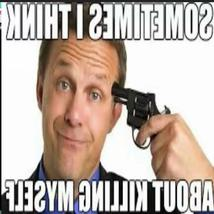
\includegraphics[width=0.7\textwidth]{figure/horizontal_flip.jpg}
        \caption{Gambar setelah \textit{flip horizontal}}
        \label{fig:gambar_flip}
    \end{subfigure}

    \caption{Perbandingan Gambar Augmentasi \textit{Flip Horizontal}}
    \label{fig:perbandingan_flip}
\end{figure}


\subsubsection{\textit{Rotation}} \label{subsubsubsec:rotation}
Selain \textit{flipping horizontal}, \textit{rotasi acak} juga diterapkan pada gambar. Pada tahap ini, gambar diputar secara acak dengan rotasi sebesar $15^\circ$. Dengan menambahkan rotasi acak, model dapat meningkatkan ketahanannya terhadap perubahan orientasi gambar. Contoh dari augmentasi ini dapat dilihat pada Gambar \ref{fig:perbandingan_rotasi}, yang menunjukkan perbandingan antara gambar asli dan hasil augmentasi rotasi.

\begin{figure}[H]
    \centering
    % Gambar 1: Asli
    \begin{subfigure}[b]{0.45\textwidth}
        \centering
        
\includegraphics[width=0.7\textwidth]{figure/gambarasli.jpg}
        \caption{Gambar asli}
        \label{fig:gambar_asli_rotation}
    \end{subfigure}
    \hspace{0.05\textwidth}
    % Gambar 2: Rotasi
    \begin{subfigure}[b]{0.45\textwidth}
        \centering
        
\includegraphics[width=0.7\textwidth]{figure/rotation.jpg}
        \caption{Gambar setelah \textit{rotasi}}
        \label{fig:gambar_rotasi}
    \end{subfigure}

    \caption{Perbandingan Gambar Augmentasi \textit{Rotasi Acak}}
    \label{fig:perbandingan_rotasi}
\end{figure}


\subsubsection{\textit{Color Jitter}} \label{subsubsubsec:color_jitter}
 \textit{Color jitter}juga diterapkan pada gambar untuk meningkatkan ketahanan model terhadap variasi pencahayaan dan warna. Pada tahap ini, kecerahan  kontras, dan saturasi diubah secara acak dengan nilai 0,2 sedangkan rona diubah secara acak 0,1. Teknik ini bertujuan untuk memperkaya variasi gambar dalam dataset, sehingga model dapat belajar mengenali objek dengan lebih baik meskipun dalam kondisi pencahayaan yang berbeda atau variasi warna yang bervariasi. Contoh dari augmentasi ini dapat dilihat pada Gambar \ref{fig:perbandingan_colorjitter}, yang menunjukkan perbandingan antara gambar asli dan hasil augmentasi \textit{color jitter}.

\begin{figure}[H]
    \centering
    % Gambar 1: Asli
    \begin{subfigure}[b]{0.45\textwidth}
        \centering
        
\includegraphics[width=0.7\textwidth]{figure/gambarasli.jpg}
        \caption{Gambar asli}
        \label{fig:gambar_asli_color_jitter}
    \end{subfigure}
    \hspace{0.05\textwidth}
    % Gambar 2: Color Jitter
    \begin{subfigure}[b]{0.45\textwidth}
        \centering
        
\includegraphics[width=0.7\textwidth]{figure/colorjitter.jpg}
        \caption{Gambar setelah \textit{color jitter}}
        \label{fig:gambar_colorjitter}
    \end{subfigure}

    \caption{Perbandingan Gambar Augmentasi \textit{Color Jitter}}
    \label{fig:perbandingan_colorjitter}
\end{figure}

\subsection{\textit{Pre-processing} oleh Model} \label{subsec:preprocessing_oleh_model}
Selain \textit{pre-processing} yang dilakukan secara langsung melalui augmentasi data, sebagian tahapan \textit{pre-processing} juga dilakukan secara otomatis oleh model yang digunakan dalam penelitian ini. Pada modalitas teks, proses seperti tokenisasi, normalisasi huruf, serta pemetaan teks menjadi representasi numerik dilakukan oleh \textit{tokenizer} ELECTRA sebagai bagian dari \textit{pipeline} model. Pada tahap bagian ini, panjang maksimum \textit{input} teks dibatasi hingga 128 token. Pemilihan ini berdasarkan analisis dataset, mayoritas teks pada meme memiliki panjang yang relatif pendek dan tidak melebihi batas tersebut, sehingga tidak diperlukan proses tambahan.Sementara itu, pada modalitas gambar, normalisasi nilai piksel dilakukan secara otomatis oleh \textit{CLIP processor}. Proses ini mencakup standarisasi nilai piksel sesuai dengan parameter yang digunakan pada pelatihan model CLIP, sehingga data yang masuk telah sesuai dengan kebutuhan arsitektur model.

Dengan demikian, sebagian besar proses \textit{pre-processing} tidak dilakukan secara manual oleh peneliti, melainkan terintegrasi langsung dalam \textit{pipeline} model. Pendekatan ini memastikan bahwa data yang digunakan dalam pelatihan telah berada dalam format yang optimal tanpa memerlukan tahap pemrosesan tambahan. Selain itu, dengan memanfaatkan kemampuan \textit{pre-processing} otomatis dari model, penelitian ini dapat lebih fokus pada pengembangan arsitektur multimodal serta analisis hasil, tanpa harus terlibat dalam proses \textit{pre-processing} yang kompleks secara manual.


\subsection{Pengembangan Model } \label{subsec:pengembangan_model}
Berikut adalah tahapan dalam pengembangan model arsitektur multimodal dengan menggunakan penggabungan fitur dalam tingkat menengah \textit{intermediate fusion} \par
\begin{figure}[H]
	\centering
	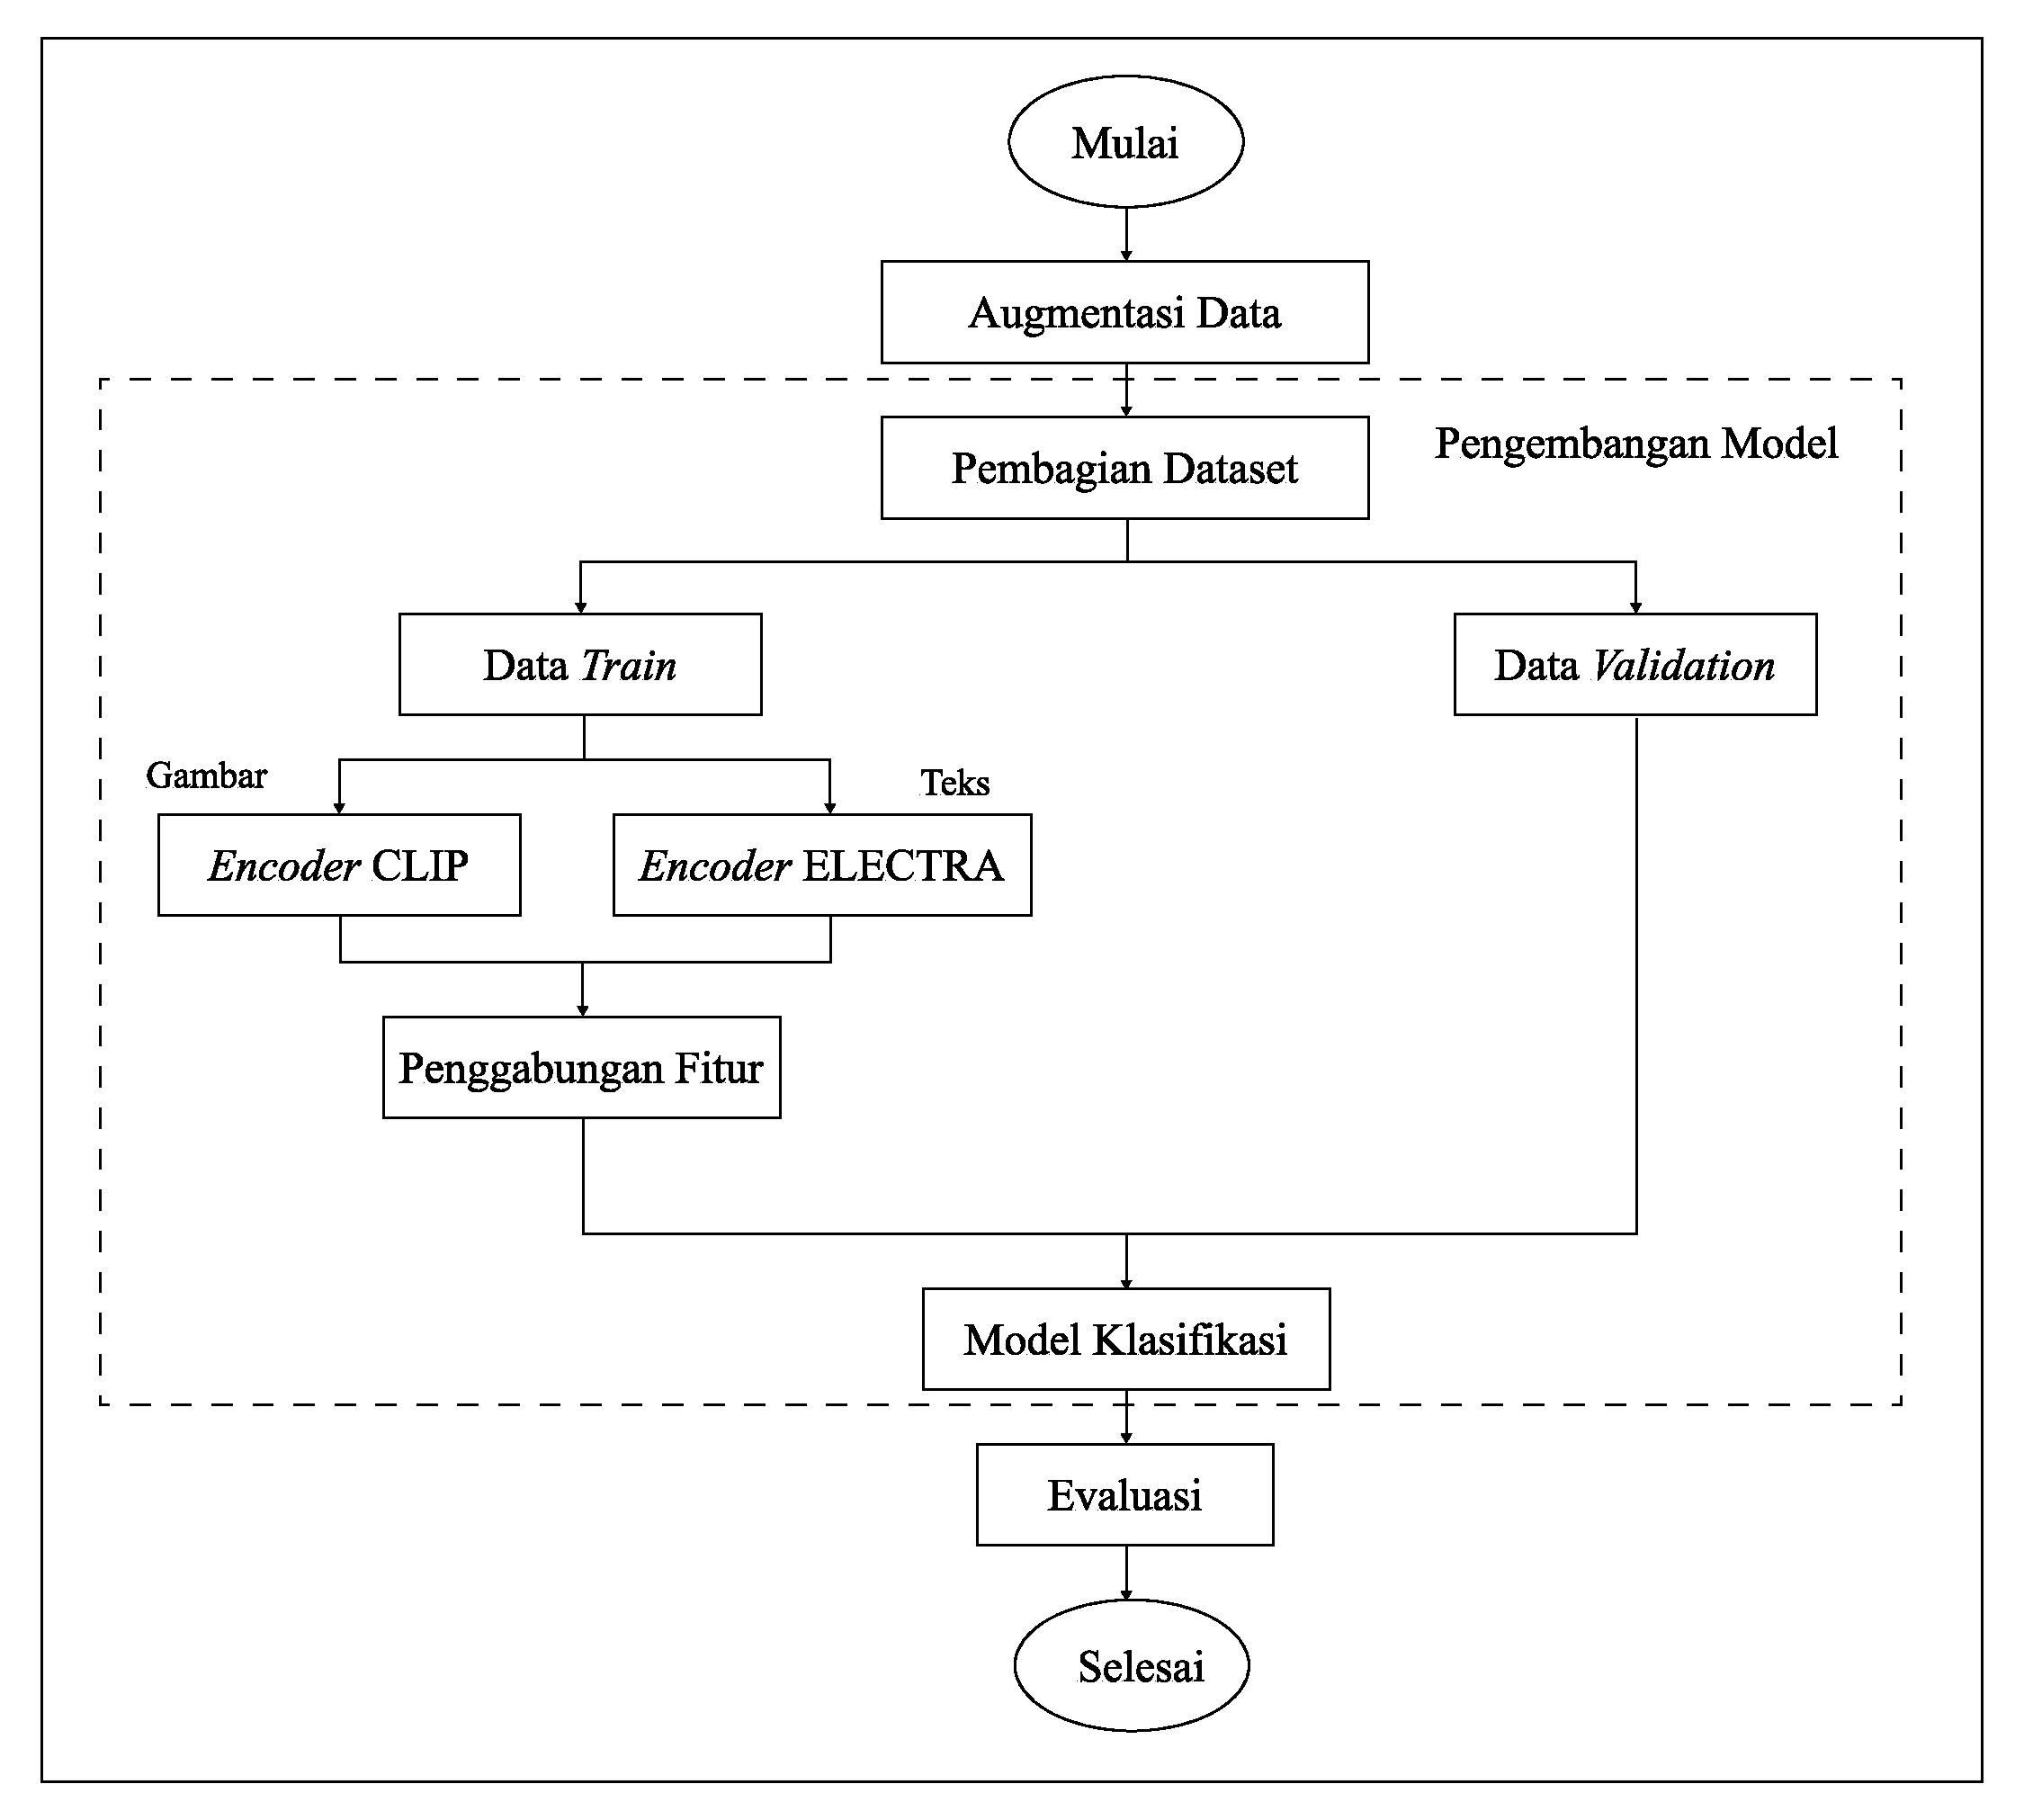
\includegraphics[width=1\textwidth]{figure/flowcharttt.pdf}
	\caption{Alur Pengembangan Model}
	\label{fig:pengembangan_model}
	% {\footnotesize Sumber: Vaswani et al., 2017}
\end{figure}
\par

\subsubsection{Pembagian Data} \label{subsubsec:pembagian_data}
Data yang telah melalui tahap \textit{pre-processing} selanjutnya dibagi dengan rasio 80:20 menggunakan metode \textit{stratified split} untuk menjaga distribusi kelas tetap seimbang. Sebanyak 80\% dari total data digunakan sebagai data latih untuk proses pembelajaran model, sedangkan 20\% sisanya digunakan sebagai data validasi. Pembagian ini bertujuan untuk memastikan bahwa model memperoleh jumlah data yang cukup untuk mempelajari pola fitur multimodal secara optimal, sekaligus menyediakan data yang representatif untuk mengevaluasi kinerja model selama proses pelatihan tanpa terjadi kebocoran data. Selain itu, penerapan \textit{stratified split} berdasarkan label memastikan bahwa proporsi kelas \textit{self-harm} dan \textit{non self-harm} tetap terjaga pada data latih dan validasi.

\subsubsection{Pelatihan model} \label{subsubsec:pelatihan_model}
Tahap pelatihan model dilakukan dengan arsitektur \textit{dual-encoder} yang menggabungkan dua modalitas input. Ekstraksi fitur visual dalam penelitian ini menggunakan model \textit{Contrastive Language-Image Pre-training} (CLIP) varian CLIP ViT \textit{base} \textit{patch-size} 32 dengan parameter ~110 juta. Pemilihan CLIP didasarkan pada efektivitasnya yang telah terbukti dalam studi literatur terdahulu, seperti pada \textit{framework} MOMENTA dan Hate-CLIPper, dimana representasi visual CLIP terbukti krusial dalam menangkap hubungan semantik lintas-modalitas dan mengenali konten implisit tanpa memerlukan arsitektur yang terlalu kompleks \cite{pramanick2021momenta} \cite{kumar2022hateclipper}. 

CLIP digunakan secara spesifik sebagai \textit{encoder} untuk modalitas gambar, dengan hanya memanfaatkan komponen \textit{vision encoder} tanpa melibatkan \textit{text encoder} CLIP. Pendekatan ini bertujuan untuk memperoleh representasi visual yang kaya dan kontekstual dari gambar, yang kemudian dikombinasikan dengan representasi dari modalitas teks pada tahap selanjutnya. Penggunaan \textit{vision encoder} CLIP secara terpisah juga telah banyak diterapkan dalam penelitian sebelumnya, yang menunjukkan bahwa fitur visual dari CLIP tetap memiliki performa yang kuat meskipun digunakan secara independen dari arsitektur multimodal aslinya \cite{gao2021clipadapter}. Selain itu, pada penelitian ini model CLIP difungsikan murni sebagai \textit{feature extractor} tanpa dilakukan proses \textit{fine-tuning}. Dengan demikian, seluruh parameter pada \textit{vision encoder} dibekukan (\textit{frozen}) selama proses pelatihan, sehingga model hanya berperan dalam mengekstraksi fitur visual yang stabil dan telah terlatih sebelumnya.

Penelitian ini menggunakan model ELECTRA varian \textit{Suicidality-ELECTRA} yang telah dilatih sebelumnya (\textit{pretrained}) untuk mendeteksi kecenderungan \textit{suicidal} dalam teks. Model \textit{Suicidality-ELECTRA} dikembangkan melalui proses \textit{fine-tuning} pada berbagai dataset yang berisi teks \textit{suicidal} dan \textit{non-suicidal} yang dikumpulkan dari berbagai sumber, seperti Reddit, Twitter, serta kumpulan catatan bunuh diri dan ekspresi ideasi \textit{suicidal}. Dataset tersebut telah melalui proses pembersihan dan \textit{preprocessing} untuk menghasilkan representasi bahasa yang kaya dan beragam.  Berdasarkan evaluasi pada dataset validasi, model ini menunjukkan performa yang tinggi dengan akurasi sebesar 93,94\% dan nilai \textit{F1-score} sebesar 93,27\%, yang menunjukkan kemampuannya dalam membedakan teks \textit{suicidal} dan \textit{non-suicidal} secara konsisten \cite{Dus2022SuicidalElectra}.

Penggunaan model ini dalam penelitian menjadi relevan karena terdapat keterkaitan antara ekspresi \textit{suicidal} dan \textit{self-harm} yang berada dalam spektrum \textit{distress} psikologis. Meskipun penelitian ini berfokus pada klasifikasi meme \textit{self-harm}, penggunaan model yang telah dilatih pada data \textit{suicidal} memungkinkan penangkapan sinyal linguistik yang serupa, seperti ideasi kematian, keputusasaan, dan ekspresi emosional negatif yang sering muncul secara implisit dalam meme. Dalam penelitian ini, model digunakan sebagai \textit{feature extractor} tanpa dilakukan proses \textit{fine-tuning}, sehingga seluruh parameter model dibekukan (\textit{frozen}) selama pelatihan. Pendekatan ini memungkinkan pemanfaatan representasi bahasa yang telah dipelajari sebelumnya tanpa menambah kompleksitas pelatihan model. Ringkasan spesifikasi \textit{encoder} pada masing-masing modalitas disajikan pada Tabel~\ref{tabel:spesifikasi_encoder_modalitas}.

\begin{table}[H]
    \centering
    \caption{Spesifikasi \textit{Encoder} pada Masing-Masing Modalitas}
    \label{tabel:spesifikasi_encoder_modalitas}
    \small
    \setlength{\tabcolsep}{3pt}
    \renewcommand{\arraystretch}{1.1}
    \begin{tabular}{p{1.7cm} p{3.2cm} p{3.0cm} p{2cm}}
        \hline
        \textbf{Modalitas} & \textbf{Model} & \textbf{Arsitektur} & \textbf{Jumlah Parameter} \\
        \hline
        Gambar & CLIP ViT-B/32 & Vision Transformer & $\pm$87 juta \\
        Teks & \textit{Suicidal}-ELECTRA \textit{(Pretrained)} & Transformer  & $\pm$110 juta \\
        \hline
    \end{tabular}
\end{table}


\subsection{Model Unimodal Gambar} \label{unimodal gambar}
Model \textit{unimodal image-only} pada penelitian ini dirancang untuk mengklasifikasikan meme ke dalam kelas \textit{self-harm} dan \textit{non-self-harm} hanya berdasarkan informasi visual. Model ini digunakan sebagai \textit{baseline} untuk mengevaluasi sejauh mana modalitas gambar saja mampu menangkap sinyal risiko pada meme, sebelum dibandingkan dengan model multimodal yang diusulkan. Rancangan arsitektur model ini cukup sederhana, dengan fokus utama pada ekstraksi fitur visual menggunakan CLIP \textit{vision encoder}, diikuti oleh lapisan klasifikasi yang ringan untuk menghasilkan prediksi akhir. Gambaran model \textit{unimodal image-only} dapat dilihat pada Gambar \ref{fig:unimodalimage}. 

\begin{figure}[h]
\centering
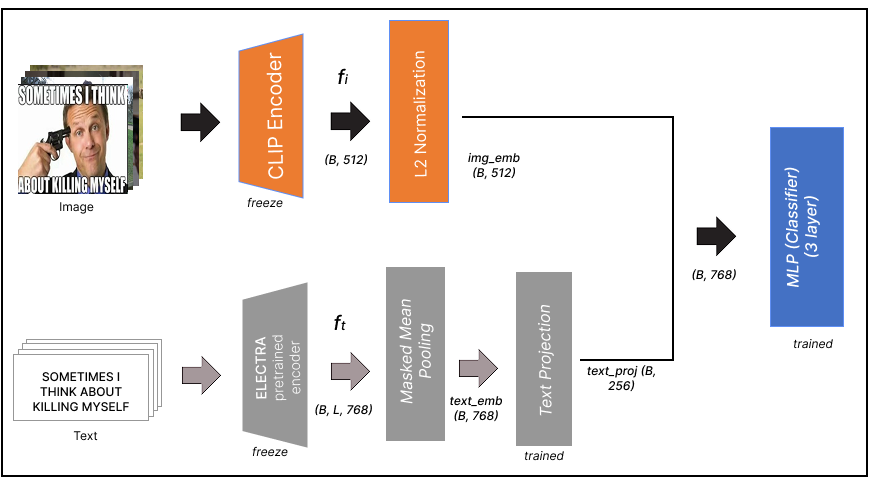
\includegraphics[width=1\textwidth]{figure/imgonly.png}
\caption{Rancangan (\textit{Unimodal Image-Only})}
\label{fig:unimodalimage}
\end{figure}

Arsitektur model memanfaatkan CLIP \textit{Vision Encoder} untuk ekstraksi fitur pada modalitas gambar. \textit{Input} citra terlebih dahulu diproses oleh \textit{encoder} visual CLIP untuk menghasilkan representasi visual berdimensi tinggi. Selanjutnya, vektor fitur visual tersebut dinormalisasi menggunakan \textit{L2 Normalization} agar representasi berada pada skala yang stabil dan konsisten sebelum diteruskan ke tahap klasifikasi. Representasi akhir kemudian menjadi \textit{input} bagi MLP \textit{classifier} 3 layer untuk menghasilkan probabilitas kelas \textit{self-harm} dan \textit{non-self-harm}.

Meskipun model ini berfokus sepenuhnya pada modalitas gambar, \textit{input} teks tetap diterima oleh fungsi model untuk menjaga kesesuaian dengan \textit{pipeline} multimodal yang sama pada proses pelatihan dan evaluasi. Namun, pada model unimodal \textit{image-only}, cabang teks tidak digunakan dalam pembentukan fitur dan diabaikan dalam proses prediksi. Pendekatan ini dipilih agar rancangan eksperimen tetap konsisten antar varian model, sekaligus memungkinkan perbandingan yang lebih adil antara model unimodal dan multimodal. Secara umum, model unimodal \textit{image-only} dirancang agar tetap ringan, sederhana, dan terfokus pada kontribusi informasi visual. Dengan menjadikan ini sebagai \textit{baseline}, penelitian ini dapat mengukur apakah representasi visual saja sudah cukup untuk mendeteksi konten \textit{self-harm}, atau apakah diperlukan penggabungan dengan modalitas teks untuk memperoleh performa yang lebih baik.

Berikut beberapa skenario eksperimen \textit{hyperparameter} pada model unimodal \textit{ image-only} untuk mencapai konfigurasi \textit{hyperparameter} optimal. Variasi \textit{hyperparameter training} difokuskan pada \textit{batch size}, \textit{epoch}, \textit{learning rate}, dan \textit{patience} pada mekanisme \textit{early stopping}. Rancangan eksperimen yang digunakan ditunjukkan pada Tabel~\ref{tabel:skenario_hyperparameter_unimodal_image_only}.

\begin{table}[H]
    \centering
    \caption{Skenario Eksperimen \textit{Hyperparameter} Model Unimodal \textit{ Image-Only}}
    \label{tabel:skenario_hyperparameter_unimodal_image_only}
    \small
    \setlength{\tabcolsep}{8pt}
    \renewcommand{\arraystretch}{1.1}
    \begin{tabular}{c c c c c}
        \hline
        \textbf{Kode Eksperimen} & \textbf{\textit{Batch Size}} & \textbf{\textit{Epoch}} & \textbf{\textit{Learning Rate}} & \textbf{\textit{Patience}} \\
        \hline
        E1 & 16 & 24 & 1e-4 & 5 \\
        E2 & 32 & 24 & 1e-5 & 5 \\
        E3 & 16 & 12 & 1e-5 & 3 \\
        E4 & 8 & 24 & 1e-4 & 5 \\
        E5 & 16 & 24 & 1e-6 & 5 \\
        \hline
    \end{tabular}
\end{table}

 Variasi nilai tersebut digunakan untuk mengamati keseimbangan antara efisiensi komputasi, kemampuan generalisasi, serta kecepatan dan kestabilan pembaruan parameter selama pelatihan. Setiap konfigurasi eksperimen kemudian dievaluasi menggunakan metrik berbasis \textit{confusion matrix}, yaitu \textit{accuracy}, \textit{precision}, \textit{recall}, dan \textit{F1-score}, serta didukung oleh indikator tambahan seperti \textit{best epoch} dan \textit{validation loss} untuk menentukan performa terbaik. Dalam penelitian ini, \textit{F1-score} digunakan sebagai metrik utama karena mampu menyeimbangkan \textit{precision} dan \textit{recall}, yang penting dalam klasifikasi konten berisiko seperti \textit{self-harm}, meskipun metrik lainnya tetap dipertimbangkan untuk memberikan evaluasi yang lebih menyeluruh.



\subsection{Model Unimodal Teks} \label{unimodal teks}
Model unimodal \textit{ text-only} pada penelitian ini dirancang untuk mengklasifikasikan meme ke dalam kelas \textit{self-harm} dan \textit{non-self-harm} hanya berdasarkan informasi tekstual. Model ini digunakan sebagai \textit{baseline} untuk mengevaluasi sejauh mana modalitas teks saja mampu menangkap sinyal risiko pada meme, sebelum dibandingkan dengan model multimodal yang diusulkan. Dengan demikian, model ini berperan penting dalam mengukur kontribusi informasi teks terhadap performa klasifikasi secara keseluruhan. Gambaran arsitektur model unimodal \textit{ text-only} dapat dilihat pada Gambar \ref{fig:unimodaltext}.

\begin{figure}[h]
\centering
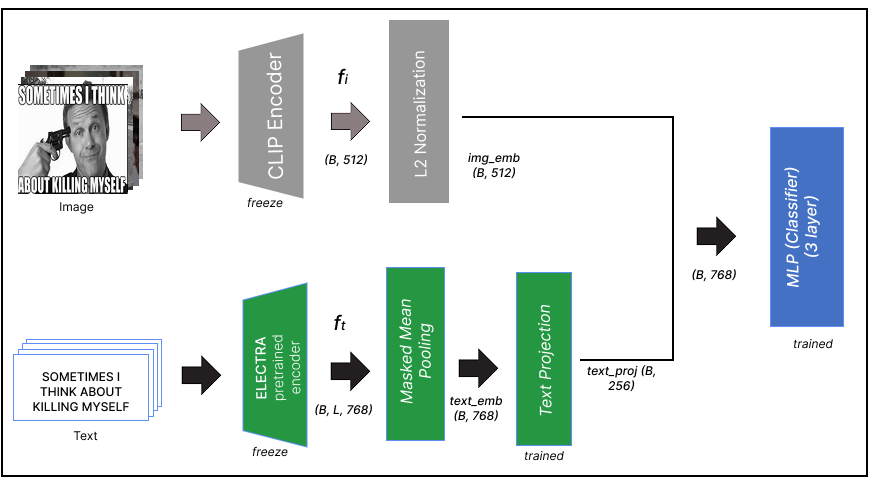
\includegraphics[width=1\textwidth]{figure/txtonly.png}
\caption{Rancangan (\textit{Unimodal Text-Only})}
\label{fig:unimodaltext}
\end{figure}


Arsitektur model memanfaatkan ELECTRA \textit{pretrained encoder} sebagai ekstraktor fitur utama pada modalitas teks. \textit{Input} teks  terlebih dahulu diproses oleh \textit{encoder} ELECTRA untuk menghasilkan representasi \textit{embedding}. Selanjutnya, representasi tersebut diringkas menggunakan \textit{masked mean pooling} untuk memperoleh representasi global dari seluruh token dalam kalimat. Representasi hasil \textit{pooling} kemudian diproyeksikan melalui \textit{text projection layer} untuk menyesuaikan dimensi fitur sebelum masuk ke tahap klasifikasi.

Berbeda dengan model multimodal, pada pendekatan ini cabang visual tetap dipertahankan dalam struktur \textit{pipeline}, namun tidak digunakan dalam proses pembentukan fitur (diabaikan). Hal ini dilakukan untuk menjaga konsistensi arsitektur dan memastikan perbandingan eksperimen yang adil antar varian model. Representasi akhir dari teks kemudian menjadi \textit{input} bagi \textit{MLP classifier} untuk menghasilkan probabilitas kelas \textit{self-harm} dan \textit{non-self-harm}. Secara umum, model unimodal \textit{ text-only} memiliki arsitektur yang sederhana dan efisien, dengan fokus utama pada pemanfaatan informasi linguistik dalam mendeteksi konten berisiko. Dengan menjadikannya sebagai \textit{baseline}, penelitian ini dapat mengevaluasi apakah informasi teks saja sudah cukup untuk mengidentifikasi meme \textit{self-harm}, atau apakah diperlukan integrasi dengan modalitas visual untuk meningkatkan performa model.

Berikut beberapa skenario eksperimen \textit{hyperparameter} pada model unimodal \textit{ text-only} untuk mencapai konfigurasi \textit{hyperparameter} optimal. Variasi \textit{hyperparameter} difokuskan pada \textit{batch size}, \textit{epoch}, \textit{learning rate}, dan \textit{patience} pada mekanisme \textit{early stopping}. Rancangan eksperimen yang digunakan ditunjukkan pada Tabel~\ref{tabel:skenario_hyperparameter_unimodal_text_only}.

\begin{table}[H]
    \centering
    \caption{Skenario Eksperimen \textit{Hyperparameter} Model Unimodal \textit{ Text-Only}}
    \label{tabel:skenario_hyperparameter_unimodal_text_only}
    \small
    \setlength{\tabcolsep}{8pt}
    \renewcommand{\arraystretch}{1.1}
    \begin{tabular}{c c c c c}
        \hline
        \textbf{Kode Eksperimen} & \textbf{\textit{Batch Size}} & \textbf{\textit{Epoch}} & \textbf{\textit{Learning Rate}} & \textbf{\textit{Patience}} \\
        \hline
        E6 & 16 & 24 & 1e-4 & 5 \\
        E7 & 32 & 24 & 1e-5 & 5 \\
        E8 & 16 & 12 & 1e-5 & 3 \\
        E9 & 8 & 24 & 1e-4 & 5 \\
        E10 & 16 & 24 & 1e-6 & 5 \\
        \hline
    \end{tabular}
\end{table}

% \subsubsection{Model Multimodal} \label{subsubsec:fusion_model}
% Penelitian ini menggunakan dua arsitektur \textit{model fusion} yang berbeda untuk menggabungkan informasi dari teks dan gambar. Kedua arsitektur ini dirancang untuk mendeteksi kecenderungan bunuh diri melalui analisis multimodal, yaitu teks dan gambar. Arsitektur yang dirancang sebagai berikut:

% \begin{figure}[h]
% \centering
% 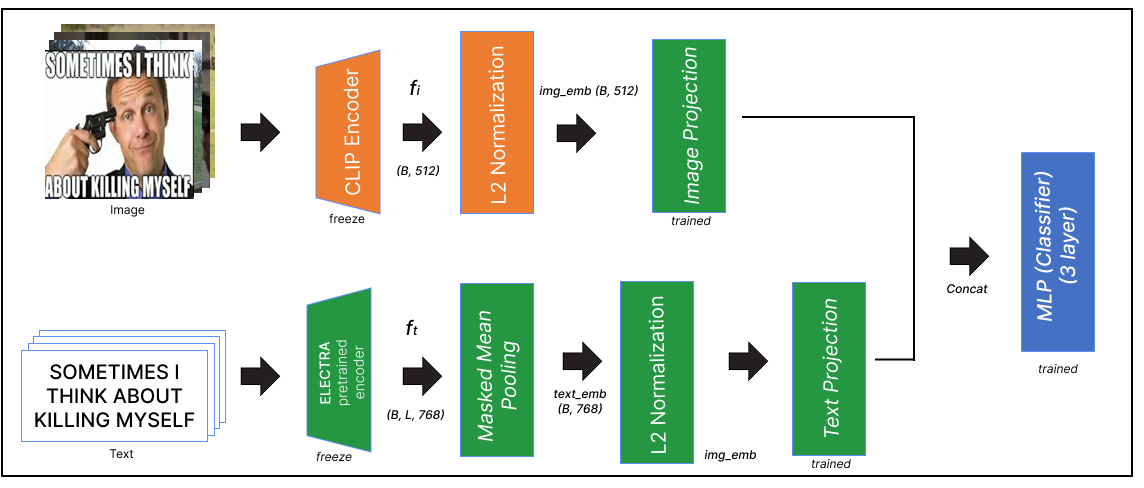
\includegraphics[width=1\textwidth]{figure/fusionmodel1.png}
% \caption{Rancangan Fusion Model Varian 1}
% \label{fig:fusion1}
% \end{figure}

% Gambar \ref{fig:fusion1} menunjukkan rancangan arsitektur fusion model varian pertama. Model ini menggunakan Transformer Encoder untuk interaksi antara modalitas teks dan gambar. Proses dimulai dengan pemrosesan gambar menggunakan CLIP \textit{encoder} untuk mengekstrak representasi fitur visual. Fitur tersebut kemudian diproyeksikan ke dalam \textit{Image Projection Layer}. Di sisi lain, teks diproses menggunakan ELECTRA \textit{pretrained encoder} yang menghasilkan representasi fitur tekstual, yang selanjutnya diproyeksikan ke dalam \textit{Text Projection Layer}.

% \textit{Projection layer} merupakan lapisan transformasi linier yang berfungsi untuk memetakan representasi fitur dari masing-masing \textit{encoder} ke dalam ruang vektor dengan dimensi yang sama, sehingga memungkinkan proses penggabungan antar-modalitas dilakukan secara efektif. Penggunaan \textit{projection layer} dalam model multimodal telah banyak digunakan untuk menyelaraskan representasi lintas-modalitas, seperti pada model CLIP yang memproyeksikan \textit{embedding} gambar dan teks ke ruang bersama untuk menghitung kesamaan semantik \cite{Radford2021CLIP}. Setelah melalui \textit{projection layer}, fitur dari teks dan gambar digabungkan dan terdapat \textit{positional embedding} untuk mempertahankan informasi urutan dan posisi. Selanjutnya, representasi gabungan tersebut diproses melalui \textit{Transformer Encoder} yang memungkinkan model untuk memahami hubungan kontekstual dan interaksi kompleks antara kedua modalitas. Hasil dari proses ini kemudian diteruskan ke \textit{Multi-Layer Perceptron} (MLP) untuk melakukan klasifikasi akhir. Arsitektur ini dirancang untuk memanfaatkan kekuatan Transformer dalam menangkap hubungan lintas-modalitas, sehingga diharapkan dapat meningkatkan kemampuan model dalam mengenali pola yang kompleks pada meme \textit{self-harm}.

% \begin{figure}[h]
% \centering
% 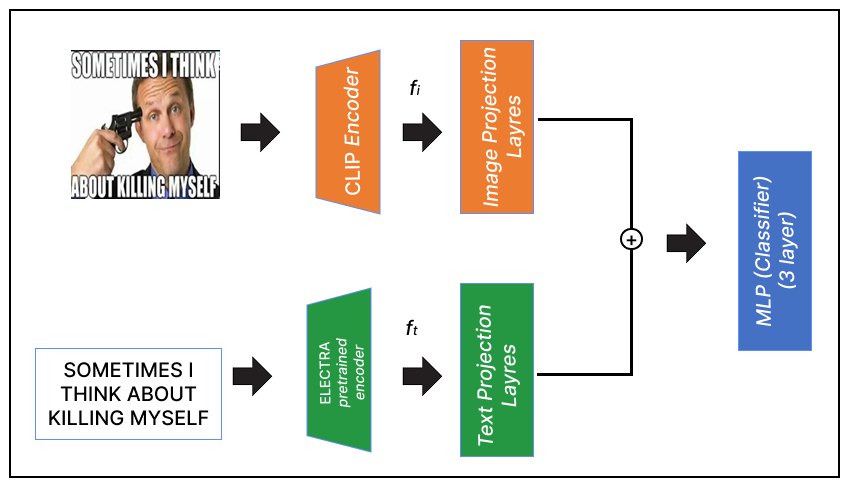
\includegraphics[width=0.9\textwidth]{figure/fusionmodel2.png}
% \caption{Rancangan Fusion Model Varian 2}
% \label{fig:fusion2}
% \end{figure}

% Gambar \ref{fig:fusion2} menunjukkan rancangan arsitektur fusion model varian kedua. Berbeda dengan varian pertama, model ini tidak menggunakan Transformer Encoder untuk interaksi antar-modalitas. Melainkan langsung menggabungkan fitur teks dan gambar untuk masuk ke MLP. Pendekatan ini menghasilkan arsitektur yang lebih sederhana dibandingkan varian pertama karena tidak melibatkan mekanisme perhatian (attention) antar-modalitas. Meskipun demikian, model ini tetap memanfaatkan representasi fitur yang kaya dari CLIP dan ELECTRA, serta menggunakan \textit{projection layer} untuk menyelaraskan dimensi fitur sebelum digabungkan. Arsitektur ini dirancang untuk memberikan baseline yang lebih sederhana dalam menggabungkan informasi dari kedua modalitas, sehingga dapat digunakan sebagai pembanding untuk mengevaluasi efektivitas penggunaan Transformer Encoder dalam varian pertama. Dengan demikian, kedua arsitektur ini memungkinkan analisis komparatif mengenai dampak kompleksitas arsitektur terhadap kinerja model dalam mendeteksi meme \textit{self-harm}.

\subsection{Model Multimodal} \label{subsubsec:fusion_model}
Model multimodal dalam penelitian ini dikembangkan dalam dua varian arsitektur, yaitu arsitektur dasar berbasis \textit{simple fusion} dan arsitektur yang dikembangkan dengan penambahan \textit{Transformer Encoder}. Kedua varian ini digunakan untuk menganalisis pengaruh mekanisme \textit{fusion} terhadap performa model dalam menangkap hubungan antar-modalitas. Pada varian pertama, arsitektur multimodal menggunakan pendekatan \textit{simple fusion}, di mana fitur teks dan gambar digabungkan menggunakan metode \textit{concatenation} dan langsung diteruskan ke \textit{Multi-Layer Perceptron} , rancangan model dapat dilihat pada Gambar \ref{fig:fusion1}.

\begin{figure}[h]
\centering
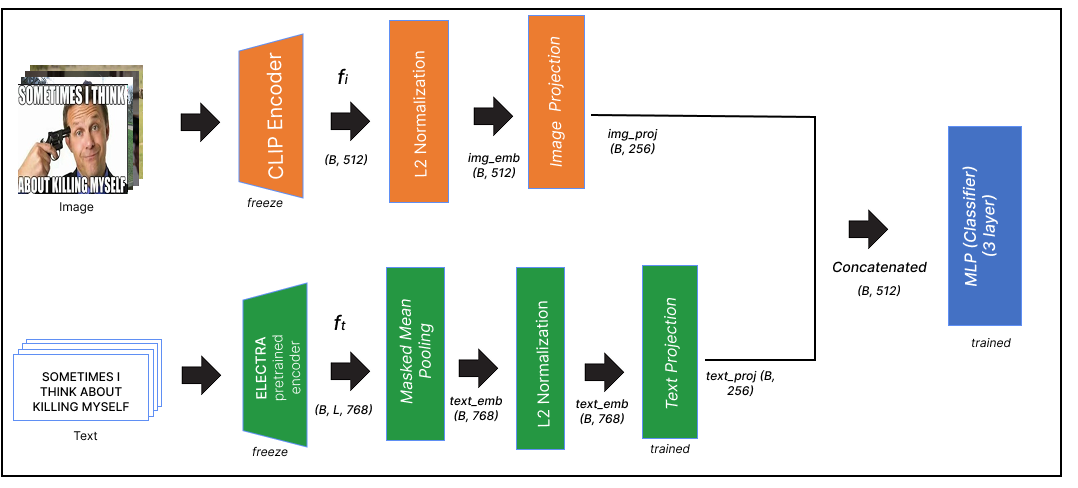
\includegraphics[width=1\textwidth]{figure/arsitekturA.png}
\caption{Rancangan Fusion Model Multimodal}
\label{fig:fusion1}
\end{figure}

Arsitektur model mengadopsi pendekatan \textit{dual-encoder}, di mana masing-masing modalitas diproses secara terpisah sebelum digabungkan pada tahap \textit{fusion}. Pada modalitas gambar, \textit{input} gambar diproses menggunakan CLIP \textit{Vision Encoder} untuk menghasilkan representasi visual berdimensi tinggi. Fitur visual tersebut kemudian dinormalisasi menggunakan \textit{L2 Normalization} untuk memastikan stabilitas representasi yang selanjutnya diproyeksikan melalui \textit{text projection layer}. Pada modalitas teks, data teks diproses menggunakan ELECTRA \textit{pretrained encoder} untuk menghasilkan \textit{embedding} kontekstual. Representasi tersebut kemudian diringkas menggunakan \textit{masked mean pooling} untuk memperoleh representasi global, yang selanjutnya diproyeksikan melalui \textit{text projection layer}. Proses ini bertujuan untuk memetakan kedua modalitas ke dalam ruang representasi yang selaras, sehingga proses \textit{fusion} dapat dilakukan secara lebih efektif. Selain itu, \textit{projection layer} juga membantu model dalam menyelaraskan distribusi fitur dari kedua modalitas yang berbeda, sehingga meningkatkan kualitas representasi multimodal yang dihasilkan.

Setelah kedua modalitas berada dalam ruang representasi yang selaras, dilakukan proses \textit{fusion} untuk menggabungkan fitur teks dan gambar. Pada arsitektur dasar, metode \textit{fusion} yang digunakan adalah \textit{concatenation}, yaitu dengan menggabungkan kedua vektor fitur menjadi satu representasi multimodal. Representasi gabungan ini kemudian diteruskan ke \textit{Multi-Layer Perceptron} \textit{classifier} yang terdiri dari tiga lapisan \textit{fully connected} untuk menghasilkan probabilitas kelas akhir. Pendekatan ini memungkinkan model untuk memanfaatkan keunggulan masing-masing \textit{encoder} dalam menangkap pola visual dan linguistik, sekaligus mempelajari hubungan antar-modalitas melalui proses \textit{fusion}. Dengan demikian, model multimodal diharapkan mampu memberikan performa yang lebih baik dibandingkan model unimodal dalam mendeteksi konten \textit{self-harm}.

Eksperimen pertama pada model multimodal dilakukan dengan memvariasikan dimensi fitur dari masing-masing modalitas untuk mengevaluasi pengaruh ukuran representasi terhadap performa model. Pada eksperimen ini, \textit{hyperparameter} pelatihan menggunakan konfigurasi terbaik yang diperoleh dari eksperimen model unimodal sebelumnya, sehingga fokus analisis hanya pada pengaruh dimensi fitur. Variasi dimensi dilakukan pada hasil \textit{projection layer} baik untuk teks maupun gambar, dengan kombinasi dapat dilihat pada Tabel~\ref{tabel:variasi_dimensi_fitur_multimodal}.

\begin{table}[H]
    \centering
    \caption{Skenario Eksperimen Dimensi Fitur Model Multimodal}
    \label{tabel:variasi_dimensi_fitur_multimodal}
    \small
    \setlength{\tabcolsep}{8pt}
    \renewcommand{\arraystretch}{1.1}
    \begin{tabular}{c c c}
        \hline
        \textbf{Kode Eksperimen} & \textbf{Dimensi Teks} & \textbf{Dimensi Gambar} \\
        \hline
        E11 & 768 & 512 \\
        E12 & 768 & 256 \\
        E13 & 512 & 512 \\
        E14 & 512 & 256 \\
        E15 & 256 & 512 \\
        E16 & 256 & 256 \\
        \hline
    \end{tabular}
\end{table}

Setelah diperoleh kombinasi dimensi fitur terbaik, eksperimen dilanjutkan dengan mengevaluasi berbagai strategi untuk menangani ketidakseimbangan kelas (\textit{class imbalance}). Pada tahap ini, \textit{hyperparameter} pelatihan tetap menggunakan konfigurasi terbaik sebelumnya, sedangkan variasi dilakukan pada fungsi \textit{loss} yang digunakan. Eksperimen ini mencakup penggunaan \textit{weighted cross-entropy loss} untuk memberikan bobot lebih pada kelas minoritas, serta penerapan teknik \textit{focal loss} yang dirancang untuk mengatasi ketidakseimbangan dengan memfokuskan pembelajaran pada contoh yang sulit diklasifikasikan. Pendekatan ini bertujuan untuk meningkatkan sensitivitas model terhadap kelas minoritas, khususnya dalam mendeteksi konten \textit{self-harm}, sehingga dapat meminimalkan kesalahan prediksi \textit{false negative}. Hasil terbaik dari eksperimen ini akan digunakan sebagai konfigurasi dasar pada tahap eksperimen berikutnya. Rancangan eksperimen untuk strategi penanganan ketidakseimbangan kelas dapat dilihat pada Tabel~\ref{tabel:strategi_penanganan_imbalance_multimodal}.

\begin{table}[H]
    \centering
    \caption{Skenario Eksperimen Strategi \textit{Loss} pada Model}
    \label{tabel:strategi_penanganan_imbalance_multimodal}
    \small
    \setlength{\tabcolsep}{8pt}
    \renewcommand{\arraystretch}{1.1}
    \begin{tabular}{c c}
        \hline
        \textbf{Kode Eksperimen} & \textbf{\textit{Strategy Loss}} \\
        \hline
        E17 & \textit{Class Weight} (\textit{Cross Entropy Loss}) \\
        E18 & \textit{Focal Loss} ($\gamma = 2{,}0$) \\
        E19 & \textit{Class Weight} + \textit{Focal Loss} ($\gamma = 2{,}0$) \\
        \hline
    \end{tabular}
\end{table}

Eksperimen yang dilakukan selanjutnya untuk mengevaluasi berbagai metode \textit{fusion} dalam menggabungkan representasi fitur teks dan gambar. Pada tahap ini, digunakan kombinasi dimensi terbaik dan strategi penanganan ketidakseimbangan kelas terbaik dari eksperimen sebelumnya, sehingga analisis difokuskan pada pengaruh metode \textit{fusion} terhadap performa model. Eksperimen ini bertujuan untuk mengidentifikasi metode \textit{fusion} yang paling efektif dalam menangkap hubungan antar-modalitas. Metode yang lebih kompleks seperti \textit{attention} dan \textit{bilinear fusion} diharapkan mampu memodelkan interaksi yang lebih kaya antara teks dan gambar dibandingkan metode sederhana seperti \textit{concatenation} atau \textit{addition}. Rancangan eksperimen untuk metode \textit{fusion} dapat dilihat pada Tabel~\ref{tabel:metode_fusion_multimodal}.
\begin{table}[H]
    \centering
    \caption{Skenario Eksperimen Metode \textit{Fusion} pada Model Multimodal}
    \label{tabel:metode_fusion_multimodal}
    \small
    \setlength{\tabcolsep}{8pt}
    \renewcommand{\arraystretch}{1.1}
    \begin{tabular}{c c}
        \hline
        \textbf{Kode Eksperimen} & \textbf{Metode Fusion} \\
        \hline
        E20 & \textit{Concatenate} \\
        E21 & \textit{Addition (Sum)} \\
        E22 & \textit{Multiplication} \\
        E23 & \textit{Gated Fusion} \\
        E24 & \textit{Attention Fusion} \\
        E25 & \textit{Bilinear Fusion} \\
        \hline
    \end{tabular}
\end{table}

Pada varian kedua, dilakukan pengembangan arsitektur dengan menambahkan \textit{Transformer Encoder} sebanyak dua layer sebelum representasi fitur diteruskan ke tahap klasifikasi menggunakan MLP (\textit{Multi-Layer Perceptron}). Penambahan lapisan ini bertujuan untuk interaksi lintas-modalitas (\textit{cross-modality interaction}) antara fitur gambar dan teks secara lebih mendalam. Dengan memanfaatkan mekanisme \textit{self-attention} pada Transformer, model dapat menangkap hubungan kontekstual antar fitur dari kedua modalitas secara dinamis, sehingga diharapkan mampu meningkatkan kualitas representasi multimodal yang dihasilkan. Ilustrasi arsitektur model yang digunakan dalam penelitian ini dapat dilihat pada Gambar~\ref{fig:arsitektur_model}.

\begin{figure}[H]
\centering
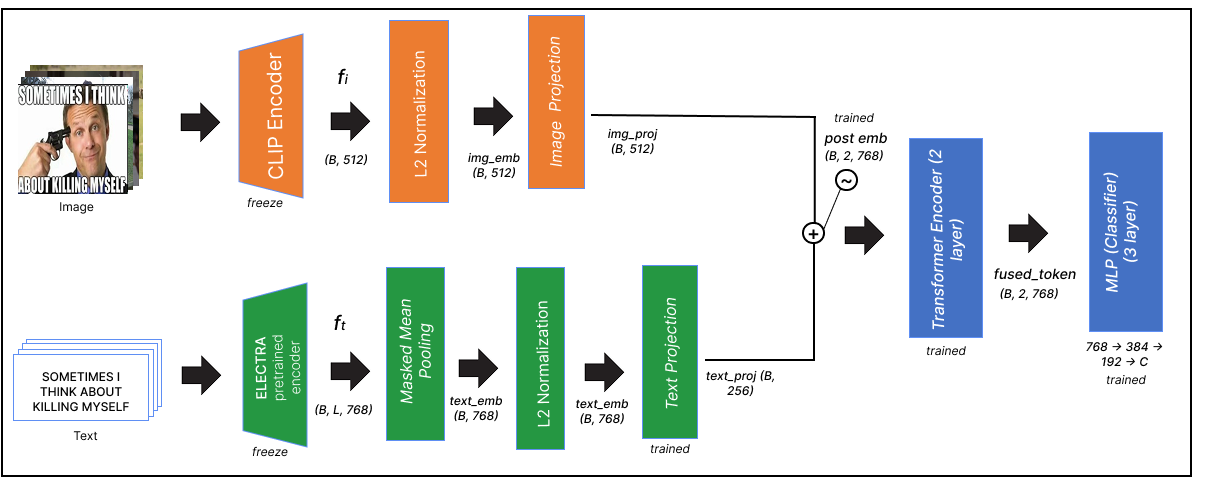
\includegraphics[width=1\textwidth]{figure/arsitekturB.png}
\caption{Rancangan Arsitektur Model Multimodal dengan Transformer Encoder}
\label{fig:arsitektur_model}
\end{figure}

Selanjutnya, untuk mengevaluasi pengaruh representasi multimodal yang dihasilkan oleh arsitektur tersebut, dilakukan eksperimen dengan memvariasikan \textit{positional encoding} dari urutan fitur teks dan gambar sebelum masuk ke dalam MLP. Eksperimen ini bertujuan untuk menganalisis sejauh mana urutan token multimodal mempengaruhi performa model dalam proses klasifikasi. Rancangan eksperimen yang digunakan dapat dilihat pada Tabel~\ref{tabel:positional_encoding_multimodal}.

\begin{table}[H]
    \centering
    \caption{Skenario Eksperimen \textit{Positional Encoding} pada Model Multimodal}
    \label{tabel:positional_encoding_multimodal}
    \small
    \setlength{\tabcolsep}{8pt}
    \renewcommand{\arraystretch}{1.1}
    \begin{tabular}{c c}
        \hline
        \textbf{Kode Eksperimen} & \textbf{\textit{Positional Encoding}} \\
        \hline
        E26 & [\textit{Image}, \textit{Text}] \\
        E27 & [\textit{Text}, \textit{Image}] \\
        \hline
    \end{tabular}
\end{table}



\subsection{Evaluasi Model} \label{subsec:evaluasi_model}
Evaluasi kinerja model dalam penelitian ini dilakukan menggunakan metrik standar yang diturunkan dari \textit{confusion matrix}, yaitu \textit{accuracy}, \textit{precision}, \textit{recall}, dan \textit{F1-score}. Keempat metrik ini digunakan untuk memberikan gambaran menyeluruh mengenai performa model dalam mengklasifikasikan data. Namun, dalam klasifikasi konten berisiko seperti \textit{self-harm}, evaluasi tidak hanya berfokus pada \textit{accuracy} karena metrik tersebut dapat bersifat menyesatkan pada data yang tidak seimbang (\textit{imbalanced data}). Oleh karena itu,evaluasi tetap memperhatikan \textit{recall} untuk meminimalkan kesalahan \textit{false negative}, yaitu kondisi di mana konten berbahaya tidak terdeteksi oleh sistem, serta \textit{precision} untuk memastikan bahwa prediksi positif yang dihasilkan benar-benar relevan.

Sebagai metrik utama, \textit{F1-score} digunakan karena mampu menyeimbangkan antara \textit{precision} dan \textit{recall}, sehingga memberikan evaluasi yang lebih representatif dalam kasus klasifikasi dengan risiko tinggi. Penggunaan \textit{F1-score} sebagai metrik utama dalam deteksi konten berbahaya juga didukung oleh penelitian sebelumnya yang menunjukkan bahwa keseimbangan antara \textit{false positive} dan \textit{false negative} sangat krusial dalam sistem deteksi konten sensitif dan berisiko \cite{Sokolova2009Performance} \cite{Sharma2022HarmfulMemes}. Dengan demikian, meskipun seluruh metrik evaluasi tetap dipertimbangkan, \textit{F1-score} menjadi indikator utama dalam menilai keandalan model, karena mampu merepresentasikan performa model secara lebih komprehensif dalam mengklasifikasikan konten multimodal yang kompleks dan berisiko.


\subsection{Evaluasi oleh \textit{Annotator} Manusia} \label{subsec:evaluasi_annotator_manusia}
Evaluasi oleh \textit{annotator} manusia dilakukan untuk membandingkan hasil prediksi model dengan interpretasi manusia terhadap data uji yang berada di luar distribusi dataset pelatihan (\textit{out-of-distribution}) sebagai upaya untuk mengukur kemampuan generalisasi model. Pendekatan ini digunakan untuk menilai sejauh mana model mampu memahami konteks multimodal yang kompleks, khususnya pada meme dengan indikasi \textit{self-harm} yang sering kali mengandung makna implisit melalui kombinasi elemen visual dan tekstual. Dalam proses ini, dua \textit{annotator} independen diminta untuk memberikan label secara terpisah terhadap sejumlah data uji, sehingga memungkinkan analisis terhadap variasi interpretasi manusia.

Tahap awal evaluasi dilakukan dengan mengukur tingkat kesepakatan antar \textit{annotator} (\textit{inter-annotator agreement}) untuk mengetahui konsistensi interpretasi manusia terhadap data. Tingkat kesepakatan ini mencerminkan sejauh mana suatu konten dapat diinterpretasikan secara seragam, serta memberikan gambaran mengenai tingkat subjektivitas dalam proses anotasi. Setelah proses anotasi selesai, dilakukan penentuan label akhir (\textit{ground truth}) berdasarkan hasil anotasi kedua \textit{annotator}. Apabila kedua \textit{annotator} memberikan label yang sama, maka label tersebut langsung digunakan sebagai \textit{ground truth}. Namun, apabila terjadi perbedaan label (\textit{disagreement}), maka dilakukan proses peninjauan ulang secara manual oleh peneliti (\textit{adjudication}) dengan mengacu pada \textit{annotation guideline} yang telah ditetapkan sebelumnya, sehingga label akhir tetap konsisten dan terstandarisasi.

Selanjutnya, hasil prediksi model dibandingkan dengan label yang telah ditetapkan oleh \textit{annotator} manusia sebagai \textit{ground truth}. Perbandingan ini bertujuan untuk mengevaluasi performa model dalam memahami konteks multimodal dibandingkan dengan interpretasi manusia. Evaluasi dilakukan menggunakan \textit{confusion matrix} untuk menghitung metrik performa seperti \textit{accuracy}, \textit{precision}, \textit{recall}, dan \textit{F1-score}. Melalui pendekatan ini, dapat diketahui sejauh mana model mampu mendeteksi konten \textit{self-harm} secara akurat, terutama pada data yang bersifat ambigu.

\subsection{Analisis Hasil dan Pembahasan} \label{subsec:analisis_hasil_dan_pembahasan}
Tahap akhir penelitian ini adalah analisis hasil dan pembahasan. Pada tahap ini, hasil evaluasi model dianalisis untuk melihat seberapa baik model dalam mengenali meme \textit{self-harm}. Analisis meliputi penjelasan metrik evaluasi, kesalahan yang terjadi, serta kelebihan dan kekurangan model. Pembahasan juga mencakup manfaat hasil penelitian dan saran untuk pengembangan selanjutnya. \par

\section{Alat dan Bahan Tugas Akhir} \label{sec:alat_dan_bahan_tugas_akhir}
Subbab ini menjelaskan perangkat lunak dan sumber daya yang digunakan dalam mendukung pelaksanaan penelitian. Perangkat yang digunakan mencakup berbagai \textit{software, library,} serta platform komputasi yang berperan dalam proses pengolahan data dan pengembangan model. Pemilihan alat dan bahan tersebut disesuaikan dengan kebutuhan penelitian, khususnya dalam pengembangan model multimodal berbasis \textit{deep learning}. Dengan demikian, penggunaan perangkat ini diharapkan dapat menunjang proses penelitian secara efektif dan efisien.

\subsection{\textit{Software dan Library}} \label{subsec:software_dan_library}
\textit{Software} dan \textit{library} yang digunakan untuk mendukung pelaksanaan penelitian ini dengan rincian sebagai berikut:
\begin{enumerate}[noitemsep]
    \item \textit{Code Editor} Visual Studio Code untuk penulisan kode program.
    \item \textit{Library Deep Learning} \textit{PyTorch} digunakan untuk implementasi dan pelatihan model.
    \item Perangkat komputer digunakan sebagai media utama dalam menjalankan eksperimen dan pelatihan model. Proses pelatihan dilakukan dengan memanfaatkan GPU NVIDIA GeForce RTX 5070.
    \item GitHub sebagai media penyimpanan repositori (\textit{repository}) dan manajemen kode.
    \item Platform desain Canva yang digunakan dalam proses pembuatan dataset meme secara manual.
\end{enumerate}

\subsection{Dataset} \label{subsec:dataset}
Dataset yang digunakan dalam penelitian ini terdiri dari dataset primer dan sekunder. Berikut komposisi \textit{dataset} awal yang digunakan dalam penelitian ini. \textit{Dataset} diperoleh dari tiga sumber utama, yaitu data  dari media sosial, data hasil rekayasa \textit{dataset}, serta meme umum dari \textit{dataset} publik sebagai pembanding. Rincian jumlah masing-masing data disajikan pada Tabel~\ref{tabel:komposisi_dataset}.

\begin{table}[H]
    \centering
    \caption{Komposisi Dataset Awal Penelitian}
    \label{tabel:komposisi_dataset}
    \small
    \setlength{\tabcolsep}{3pt}
    \renewcommand{\arraystretch}{1.1}
    \begin{tabular}{p{0.6cm} p{3.8cm} p{1.6cm} p{1.4cm}}
        \hline
        \textbf{No} & {\raggedright \textbf{Jenis Data}\par} & \textbf{Sumber Data} & \textbf{Jumlah} \\
        \hline
        1 & {\raggedright Media Sosial\par} & Primer & 268 \\
        2 & {\raggedright Rekayasa \textit{Dataset}\par} & Sekunder & 524 \\
        3 & {\raggedright Meme Umum (\textit{Dataset} Publik)\par} & Sekunder & 1.500 \\
        \hline
        & {\raggedright \textbf{Total}\par} & & \textbf{2.292} \\
        \hline
    \end{tabular}
\end{table}

\section{Ilustrasi Perhitungan Metode} \label{sec:ilustrasi_perhitungan_metode}
Pada bagian ini disajikan ilustrasi perhitungan dari metode-metode utama yang digunakan dalam penelitian. Uraian perhitungan diberikan secara bertahap agar  pembentukan nilai pada setiap metode dapat dipahami dengan lebih jelas. Ilustrasi ini mencakup perhitungan InfoNCE (\textit{contrastive loss}) yang digunakan dalam model CLIP, perhitungan \textit{Token Detection Loss} pada model ELECTRA dan perhitungan metrik evaluasi seperti \textit{precision}, \textit{recall}, dan \textit{F1-score} yang digunakan untuk mengevaluasi performa model.


\subsection{Ilustrasi Perhitungan InfoNCE} \label{subsec:ilustrasi_perhitungan_infonce}
Pada bagian ini, akan dihitung \textit{loss} menggunakan \ref{eq:clip-infoNCE}. InfoNCE digunakan untuk menghitung kesamaan antara representasi gambar dan teks. 
Misalkan terdapat dua pasangan gambar-teks sebagai berikut:
\begin{itemize}
    \item Pasangan 1: $L_1$ dengan $T_1$
    \item Pasangan 2: $L_2$ dengan $T_2$
\end{itemize}

\medskip
Nilai kesamaan kosinus (\textit{cosine similarity}) untuk setiap pasangan adalah:
\bigskip
\begin{align*}
    \cos(f_L(L_1), f_T(T_1)) &= 0{,}85 \\
    \cos(f_L(L_1), f_T(T_2)) &= 0{,}45 \\
    \cos(f_L(L_2), f_T(T_1)) &= 0{,}40 \\
    \cos(f_L(L_2), f_T(T_2)) &= 0{,}75 \\
\end{align*}
Dengan parameter suhu $\tau = 0{,}07$, nilai \textit{loss} untuk pasangan pertama $L_1, T_1$ dapat dihitung menggunakan rumus InfoNCE berikut:\\
\bigskip
\begin{align*}
\mathcal{L}_1 = - \frac{1}{2} \Bigg(
    \log \left( \frac{e^{\cos(f_L(L_1), f_T(T_1)) / \tau}}
    {\sum_{i=1}^{2} e^{\cos(f_L(L_1), f_T(T_i)) / \tau}} \right)
    + \log \left( \frac{e^{\cos(f_T(T_1), f_L(L_1)) / \tau}}
    {\sum_{i=1}^{2} e^{\cos(f_T(T_1), f_L(L_i)) / \tau}} \right)
\Bigg)\\
\end{align*}
Substitusi nilai \textit{cosine similarity}:

\begin{align*}
    \cos(f_L(L_1), f_T(T_1)) &= 0{,}85, \quad \cos(f_L(L_1), f_T(T_2)) = 0{,}45 \\
    \cos(f_T(T_1), f_L(L_1)) &= 0{,}85, \quad \cos(f_T(T_1), f_L(L_2)) = 0{,}40\\
\end{align*}

\textit{Term} pertama: \\
\begin{align*}
    \frac{\exp(0{,}85 / 0{,}07)}{\exp(0{,}85 / 0{,}07) + \exp(0{,}45 / 0{,}07)} 
    &\approx \frac{1{,}751 \times 10^5}{1{,}751 \times 10^5 + 624{,}8} \\
    &\approx 0{,}9996\\
\end{align*}

\textit{Term} kedua:\\
\begin{align*}
    \frac{\exp(0{,}85 / 0{,}07)}{\exp(0{,}85 / 0{,}07) + \exp(0{,}40 / 0{,}07)} 
    &\approx \frac{1{,}751 \times 10^5}{1{,}751 \times 10^5 + 302{,}5} \\
    &\approx 0{,}9998\\
\end{align*}

Substitusi ke dalam rumus:\\
\begin{align*}
    \mathcal{L}_1 &= - \frac{1}{2} \bigg[ \log(0{,}9996) + \log(0{,}9998)
    \bigg]\\
\end{align*}

Logaritma:\\
\begin{align*}
    \log(0{,}9996) &\approx -0{,}0004, \quad \log(0{,}9998) \approx -0{,}0002\\
\end{align*}

Hasil akhir:\\
\begin{align*}
    \mathcal{L}_1 &= - \frac{1}{2} \left[ -0{,}0004 + (-0{,}0002) \right] = 0{,}0003
\end{align*}

\subsection{Ilustrasi Perhitungan \textit{Token Detection Loss} pada ELECTRA} \label{subsec:ilustrasi_token_detection_loss_electra}

Pada bagian ini, akan dihitung \textit{loss} menggunakan \ref{eq:rtd-loss}. 
Misalkan terdapat sebuah kalimat yang terdiri dari 3 token, yaitu:
\\ 
\[
\text{Kalimat: } \{ \text{"Saya"}, \text{"pergi"}, \text{"ke"} \}
\]
\\

Kemudian, hasil generator model untuk token-token tersebut adalah:
\\
\[
\text{Hasil Generator: } \{ \text{"Saya"}, \text{"berlari"}, \text{"ke"} \}
\]
\\
Dari kalimat di atas, diketahui bahwa:
\begin{itemize}[noitemsep]
    \item Token "Saya" adalah token asli (\(y_1 = 1\)).
    \item Token "pergi" digantikan dengan token "berlari" (hasil generator), sehingga \(y_2 = 0\).
    \item Token "ke" adalah token asli (\(y_3 = 1\)).
\end{itemize}

Kemudian, probabilitas \(D(x_i)\) yang diberikan oleh diskriminator untuk setiap token adalah sebagai berikut:
\\
\[
D(\text{"Saya"}) = 0{,}95, \quad D(\text{"berlari"}) = 0{,}05, \quad D(\text{"ke"}) = 0{,}90
\]
\\
Sekarang, dapat dihitung \(\mathcal{L}_{RTD}\) untuk kalimat ini dengan menggunakan rumus yang telah diberikan.

\begin{align*}
    \mathcal{L}_{RTD} &= - \left[ y_1 \log D("Saya") + (1 - y_1) \log (1 - D("Saya")) \right. \\
    &\quad \left. + y_2 \log D("berlari") + (1 - y_2) \log (1 - D("berlari")) \right. \\
    &\quad \left. + y_3 \log D("ke") + (1 - y_3) \log (1 - D("ke")) \right] \\
    &= - \left[ 1 \cdot \log(0{,}95) + 0 \cdot \log(1 - 0{,}95) \right. \\
    &\quad \left. + 0 \cdot \log(0{,}05) + 1 \cdot \log(1 - 0{,}05) \right. \\
    &\quad \left. + 1 \cdot \log(0{,}90) + 0 \cdot \log(1 - 0{,}90) \right]\\
\end{align*}

Setelah mengganti nilai logaritma:

\begin{align*}
    \mathcal{L}_{RTD} &= - \left[ \log(0{,}95) + \log(0{,}95) + \log(0{,}90) \right] \\
    &= - \left[ -0{,}0223 + -0{,}0223 + -0{,}1054 \right] \\
    &= 0{,}15 \\
\end{align*}

Dengan demikian, nilai dari \(\mathcal{L}_{RTD}\) untuk kalimat ini adalah 0,15.

\subsection{Ilustrasi Perhitungan Metrik Evaluasi} \label{subsec:ilustrasi_perhitungan_metrik_evaluasi}

Berikut ilustrasi perhitungan metrik evaluasi pada \ref{eq:accuracy}, \ref{eq:precision}, \ref{eq:recall}, dan \ref{eq:f1-score}.

Misalkan terdapat hasil pengujian model dengan jumlah sebagai berikut:
\begin{itemize}[noitemsep]
    \item \(TP = 50\)
    \item \(TN = 40\)
    \item \(FP = 10\)
    \item \(FN = 5\)
\end{itemize}
Dengan nilai-nilai tersebut, metrik evaluasi dapat dihitung sebagai berikut:

\begin{align*}
    \textit{Accuracy} &= \frac{TP + TN}{TP + TN + FP + FN} \\
    &= \frac{50 + 40}{50 + 40 + 10 + 5} \\
    &= \frac{90}{105} \\
    &= 0{,}8571\\
\end{align*}

Jadi, \(\textit{Accuracy} = 0{,}8571\) atau 85,71\%.

\begin{align*}
    \textit{Precision} &= \frac{TP}{TP + FP} \\
    &= \frac{50}{50 + 10} \\
    &= \frac{50}{60} \\
    &= 0{,}8333\\
\end{align*}

Jadi, \(\textit{Precision} = 0{,}8333\) atau 83,33\%.


\begin{align*}
    \textit{Recall} &= \frac{TP}{TP + FN} \\
    &= \frac{50}{50 + 5} \\
    &= \frac{50}{55} \\
    &= 0{,}9091\\
\end{align*}

Jadi, \(\textit{Recall} = 0{,}9091\) atau 90,91\%.


\begin{align*}
    \textit{F1} &= 2 \times \frac{\textit{Precision} \times \textit{Recall}}{\textit{Precision} + \textit{Recall}} \\
    &= 2 \times \frac{0{,}8333 \times 0{,}9091}{0{,}8333 + 0{,}9091} \\
    &= 2 \times \frac{0{,}7562}{1{,}7424} \\
    &= 2 \times 0{,}4330 \\
    &= 0{,}8660\\
\end{align*}

Jadi, \(\textit{F1 Score} = 0{,}8660\) atau 86,60\%.

\medskip
Dari perhitungan di atas, dapat disimpulkan bahwa model memiliki:
\begin{itemize}
    \item \(\textit{Accuracy} = 85,71\%\)
    \item \(\textit{Precision} = 83,33\%\)
    \item \(\textit{Recall} = 90,91\%\)
    \item \(\textit{F1 Score} = 86,60\%\)
\end{itemize}
Metrik-metrik ini memberikan gambaran yang lebih lengkap tentang performa model dalam mengklasifikasikan data dengan benar, baik dalam hal ketepatan (\textit{precision}) maupun dalam mengidentifikasi seluruh data positif yang relevan (\textit{recall}).
\clearpage
